\documentclass[spanish,notitlepage,letterpaper,11pt]{article} % para artÌculo en castellano
\usepackage[utf8]{inputenc} % Acepta caracteres en castellano
\usepackage[T1]{fontenc} % font encoding
\usepackage[spanish]{babel}    % silabea palabras castellanas
\usepackage[none]{hyphenat} 
\usepackage{amsmath}
\usepackage{amsfonts}
\usepackage{amssymb}
\usepackage{listings}
\usepackage{subcaption}
\lstset{basicstyle=\ttfamily,
  showstringspaces=false,
  commentstyle=\color{red},
  keywordstyle=\color{blue}
}
\usepackage[colorlinks=true,urlcolor=blue,linkcolor=blue]{hyperref}% navega por el doc
\usepackage{graphicx}
\usepackage{geometry}      % See geometry.pdf to learn the layout options.
\geometry{letterpaper}                   % ... or a4paper or a5paper or ... 
%\geometry{landscape}                % Activate for for rotated page geometry
%\usepackage[parfill]{parskip}    % Activate to begin paragraphs with an empty line rather than an indent
\usepackage{epstopdf}
\usepackage{fancyhdr} % encabezados y pies de pg
\usepackage{lineno}
\usepackage{titling}
\newtheorem{myteo}{Theorem}
\newtheorem{myDef}{Definition}
\newtheorem{myAxiom}{Axiom}

\pagestyle{fancy} 
\chead{\bfseries Lectures on plasma physics} 
\lhead{} % si se omite coloca el nombre de la seccion
\rhead{26 de enero 2022} 
\lfoot{\it Jafert Serrano } 
\cfoot{UIS} 
\rfoot{\thepage} 

\voffset = -0.25in 
\textheight = 8.0in 
\textwidth = 6.5in
\oddsidemargin = 0.in
\headheight = 20pt 
\headwidth = 6.5in
\renewcommand{\headrulewidth}{0.5pt}
\renewcommand{\footrulewidth}{0,5pt}
\DeclareGraphicsRule{.tif}{png}{.png}{`convert #1 `dirname #1`/`basename #1 .tif`.png}
\numberwithin{equation}{subsection}

\begin{document}

\begin{titlepage}
\centering
\begin{minipage}{.4\textwidth}
\centering

\includegraphics[width=\linewidth]{Figures/LoGOTS.png}
\end{minipage}%
\begin{minipage}{.4\textwidth}
\centering

\includegraphics[width=\linewidth]{Figures/logouis.png}
\end{minipage}

\vspace{\baselineskip}
\rule{\textwidth}{2pt}
\vspace{\baselineskip}
\vspace{\baselineskip}
\vspace{\baselineskip}
\vspace{\baselineskip}
\vspace{\baselineskip}

\huge\textbf{LECTURES ON PLASMA PHYSICS} \\

\vspace{\baselineskip}
\vspace{\baselineskip}

\textwidth
\textbf{Miguel Jafert Serrano Mantilla}\\

\vspace{\baselineskip}
\vspace{\baselineskip}
\textit{Universidad Industrial De Santander}\\
\vspace{\baselineskip}
\textit{Grupo De Óptica Y Tratamiento De Señales}\\
\vspace{\baselineskip}
\date{31/01/2023}
\vspace{\baselineskip}


\vspace{2cm} 
\end{titlepage}

\newpage
%\title{Aqui va el nombre del proyecto}
%\author{
%\textbf{Autor \thanks{e-mail: \texttt{correo} }} \\ 
%\textit{Nombre de la institución} \\ 
%\textit{Dirección de la Institución}}
%\date{Versión $\alpha \beta$ fecha del documento }
%\maketitle
\tableofcontents

\newpage
\begin{abstract}

    
     
\end{abstract}


\section{INTRODUCTION}
    Around the $98\%$ of the visible matter is plasma, this means that a study of this matter state is really important to understand the universe and not only that, a good understanding of this phenoma will allow us to create clean sources of energy, like nuclear fusion reactors as the Tokamak, or predict high energy pehonomena that could damage the earth as the solar storms. The main idea here is to study the physics of the plasma using all the tools the physics offer, here we're gonna use classicar physics, relativistic physics, non equilibrium statistical physics and the quantum mechanics.
    
    \subsection{Definitions and general properties}

    \begin{myDef}
        Plasma: We will call plasma to a ionized gas which is made by positively charged nucleus and free electrons.
    \end{myDef}

    This definition looks very general but we must be careful, because contrary to the intuition not all the plasma are hot, there are cold plasma like the Neon gas in some fluorescent lamps and more important, how do we determine that certain gas is ionized? To answer this we must use the Saha's formula ($1982$).
    
    \subsection{Saha's formula and the ionization grade}

    \begin{figure}[h]
        \centering
        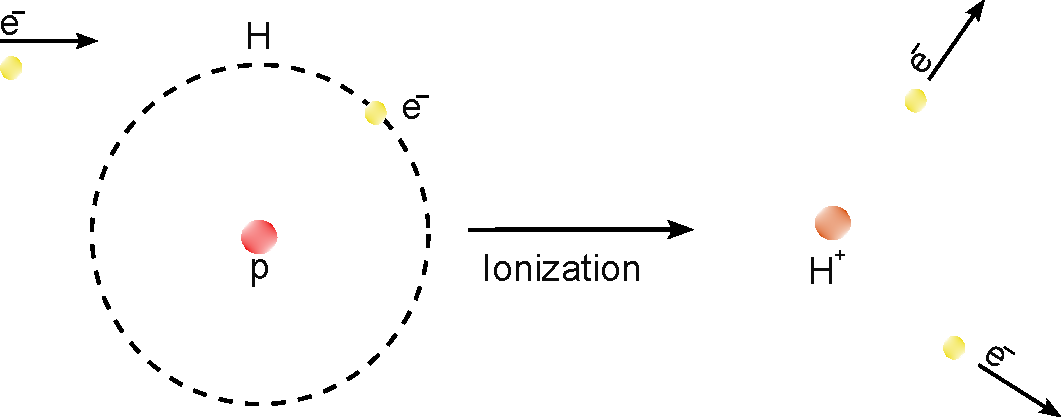
\includegraphics[width=0.8\textwidth]{Figures/Cap 1/Ionizacion.pdf}
        \caption{Hidrogen atom being ionized by the collision with an electron.}
        \label{fig:HAtm}
    \end{figure}

    To obtain the Saha's formula we must have the following considerations:

    \begin{enumerate}
        \item There are $N_{a0}$ atoms in the volumen $V$.

        \item After the ionization process there are gonna be $N_i$ ions.

        \item The system only interchange thermal energy.

        \item The number of electrons are going to be the same as the number of ions $N_{e^-} = N_i$.
    \end{enumerate}

    Due to the many particles there are in plasma a statistical treatment must be done, and due to the third consideration a canonical ensemble is gonna be used, thus the \textit{probability of finding the electron in the $k$th state.}

    \begin{equation}\label{eq:prob}
        W_k = Ae^{-\frac{E_k}{K_bT}}\;.
    \end{equation}

    Here, the $k$th energy is gonna be the energy of the $k$th level of the Hydrogen atom \ref{fig:HAtm}.

    \subsubsection{Hydrogen atom energy levels}

        There are many ways to find the mathematical expression of the energy levels of the Hydrogen atom, here we're going to use the Sommerfeld quantization, look at the appendix \ref{APX:Sommerfeld} to learn a bit more about it. For the Hydrogen atom in the figure \ref{fig:HAtm} the Hamiltonian is:

        \begin{equation}
            H = \frac{1}{2}m_ev^2 - \frac{C^2}{4\pi\epsilon_0 r}\;. \;\; [J]
        \end{equation}

        Where $C$ is the charge of the electron and $r$ the distance from the proton to the electron, before doing all the calculus this development is completely classical, the reasons to do it in this way are:
        
        \begin{itemize}
            \item It is easy.
            \item Using the quantum mechanics of the Hydrogen atom would be really long.
            \item It is easy and works perfectly.
        \end{itemize}

        So, in this classical picture the electron has got a circular motion around the proton, thus:

        \begin{equation*}
            F = m_e\frac{v^2}{r} = \frac{C^2}{4\pi\epsilon_0r^2} \rightarrow mv^2 = \frac{C^2}{4\pi\epsilon_0r}\;
        \end{equation*}

        \begin{equation}
            H = E = \frac{C^2}{8\pi\epsilon_0r} - \frac{C^2}{4\pi\epsilon_0 r} = -\frac{C^2}{8\pi\epsilon_0r}\;. \;\; [J]
        \end{equation}

        And using the Bohr's quantization of angular momentum we have $L = m_evr = k\hbar$ is easy to see:

        \begin{equation*}
            (m_evr)^2 = (k\hbar)^2 \rightarrow m_ev^2 = \frac{k^2\hbar^2}{mr^2} = \frac{C^2}{4\pi\epsilon_0r}
        \end{equation*}

        \begin{equation}\label{eq:RBoh}
            r = \frac{4\pi\hbar^2\epsilon_0k^2}{C^2m_e} \;\;[m]\;.
        \end{equation}

        The expression \ref{eq:RBoh} is known as the Bohr's radius and replacing in the energy $r$ by the equation \ref{eq:RBoh}  we will have the values for the energy in the $kth$ level:

        \begin{equation}
            E_k = -\frac{m_eC^4}{32\pi^2\epsilon_0^2\hbar^2n^2}
        \end{equation}

    When whe analyze the first energy level $k = 1$ we have got:

    \begin{equation*}
        E_1 = -\frac{m_eC^4}{32\pi^2\epsilon_0^2\hbar^2} = -\frac{\mathrm{Gm_eC^4}}{2\hbar^2} = -I\;,
    \end{equation*}

    The ionization energy for the first level is, in fact, the same in magnitude but with opposite sign, $I$ is also called the \textit{ionization potential energy} for the Hydrogen atom $I = 13.6\;[eV]$. Now, we must find the normalization constant $A$ for this we must observe the probability \ref{eq:prob} must be normalized due we have only one kind of particle so:

    \begin{equation*}
        \sum_{k}W_k = 1 = A\sum_ke^{-\frac{E_k}{K_BT}} \rightarrow A = \left[\sum_k e^{-\frac{E_k}{K_BT}} \right]^{-1}\;.
    \end{equation*}

    Lets suppose there's only one bounded state and the other not bounded, thus:

    \begin{equation}\label{eq:A}
        A = \left[e^{\frac{I}{K_BT}} + \sum_{E_k>0}e^{-\frac{E_k}{K_BT}} \right]^{-1}
    \end{equation}

    The second term is the partition function and it's summed over all the non bounded states or the continuous energy values $E_k > 0$, this partition function  allow us to calculate all the macroscopic properties of the system. \\

    To calculate that summation we must think on a phase space $(\Vec{p},\Vec{r})$ and an associated volume $(2\pi\hbar)^3$, in fact, the volume, due to the Heisenberg's indetermination principle, is $h$ the Planck's constant, but to relate it (for later) to a Fourier transforms, we write that minimum volume in terms of $\hbar$, the physics doesn't have infinitely little volumes there's a limit well imposed by the quantum mechanics laws. So our summation becomes a integral:

    \begin{equation*}
        \sum_{E_k>0} \rightarrow \int \frac{d^3pd^3r}{(2\pi\hbar)^3} \;\;\&\;\, d\tau_{min} = h^3 \;\;,\;\; d\tau = d^3pd^3r
    \end{equation*}

    Now, each electron occupies only one cell that's because they're fermions and the energy $E_k$ is continuous so we can approach it to a kinetc energy $E_k \approx \frac{P^2}{2m_e} \;[J]$ that also implies there is no interaction between the electrons and the nucleus, thus:

    \begin{equation*}
        \sum_{E_k > 0}e^{-\frac{E_k}{K_BT}} = \int \frac{e^{-\frac{p^2}{2m_eK_BT}}}{(2\pi\hbar)^3}d^3pd^3r = \frac{V}{(2\pi\hbar)^3}\int_{0}^{\infty}4\pi p^2e^{\frac{-p^2}{2m_eK_BT}}dp
    \end{equation*}

    Now to solve that integral we're gonna use a change of variables $u = \frac{p}{\sqrt{2m_eK_BT}} \;dp = \sqrt{2m_eK_BT}du$:

    \begin{equation*}
        \frac{V}{(2\pi\hbar)^3}\int_{0}^{\infty}4\pi p^2e^{\frac{-p^2}{2m_eK_BT}}dp = \frac{4\pi V}{(2\pi\hbar)^3}(2m_eK_BT)^{3/2}\int_0^{\infty}u^2e^{-u^2}du 
    \end{equation*}

    \begin{equation*}
        \frac{V}{(2\pi\hbar)^3}\int_{0}^{\infty}4\pi p^2e^{\frac{-p^2}{2m_eK_BT}}dp = \frac{4\pi V}{(2\pi\hbar)^3}(2m_eK_BT)^{3/2}\Gamma(\frac{3}{2}) = \frac{4\pi V}{(2\pi\hbar)^3}(2m_eK_BT)^{3/2}\frac{\sqrt{\pi}}{4}
    \end{equation*}

    \begin{equation*}
        \sum_{E_k > 0}e^{-\frac{E_k}{K_BT}} = V\left(\frac{m_eK_BT}{2\pi\hbar^2}\right)^{3/2} = \frac{V}{V_Q}
    \end{equation*}

    Where we can define a quantum volume related to a DeBrogli'es wave lenght like this:

    \begin{equation*}
        V_q = \left(\sqrt{\frac{2\pi}{m_eK_BT}}\hbar\right)^3 = \lambda_B^3
    \end{equation*}

    Where $\lambda_B$ is the DeBroglie's wave length and using his postulates we can find an expression for $p$ as function of the temperature:
    \begin{equation*}
        \lambda_B = \sqrt{4\pi}\frac{\hbar}{p} \rightarrow p = \sqrt{2m_eK_BT}
    \end{equation*}

    Now, we're gonna define some new densities, what we call a number density which is define as the relation between the number of something and the volume but this is for an specific volume, in this way we're gonna define the following three densities:

    \begin{enumerate}
        \item $n_e$ Density of number of electrons.
        \item $n_i$ Density of number of ions.
        \item $n_a$ Density of number of atoms.
    \end{enumerate}

    Thanks to that definitions, the physical volume is directly related to the density of number of electrons $V = n_e^{-1}$ finally, the partition function is:

    \begin{equation}\label{eq:partition}
        \sum_{E_k > 0}e^{-\frac{E_k}{K_BT}} = \frac{1}{n_e\lambda_B^3}
    \end{equation}

    Introducing \ref{eq:partition} in \ref{eq:A}:

    \begin{equation}
        A = \left[e^{\frac{I}{K_BT}} + \frac{1}{n_e\lambda_B^3}\right]^{-1}
    \end{equation}

    Let think on the probability that a proton has got a bounded electron in the first energy level $k=1$. This probability in complementary with the probability of having an ion separated by a ionization potential related with $k=1$ so $w_i = 1 - w_a$

    \begin{equation}\label{eq:ProbProt}
        w_a = \frac{e^{\frac{I}{K_BT}}}{e^{\frac{I}{K_BT}} + \frac{1}{n_e\lambda_B^3}}
    \end{equation}

    \begin{equation}\label{eq:ProbIon}
        w_i = \frac{\frac{1}{\lambda_B^3}n_e}{e^{\frac{I}{K_BT}} + \frac{1}{\lambda_B^3}n_e}
    \end{equation}

    Because there's only one type and are independent events the relation $n_i/n_1$ is $w_i/w_a$

    \begin{equation*}
        \frac{n_i}{n_a} = \frac{1}{\lambda_B^3n_e}e^{-\frac{I}{K_BT}}\;,
    \end{equation*}

    \begin{equation}\label{eq:ninena}
        \frac{n_in_e}{n_a} = \frac{e^{-\frac{I}{K_BT}}}{\lambda_B^3}\;.
    \end{equation}

    Here a first conclusion arises, \textit{the degree of ionization depends of the temperature and the electronic density}. All the mathematical development until here was using the first energy level for an Hydrogen atom, to make it worth and useful for many other plasma Saha introduced a correction. The atoms, ions an electrons have certain freedom degree $g$ generally each one has a different freedom degree, so the number density must be corrected $n \rightarrow n/g$ thus the equation \ref{eq:ninena}  becomes:

    \begin{equation}
        \frac{n_in_e}{n_a} = \frac{g_ig_e}{g_a}\frac{e^{-\frac{I}{K_BT}}}{\lambda_B^3}\;,
    \end{equation}

    \begin{equation}\label{eq:Sahas}
        \frac{n_in_e}{n_a} = \frac{g_ig_e}{g_a}\left(\frac{m_eK_B}{2\pi\hbar^2}\right)^{3/2}T^{3/2}e^{-\frac{I}{K_BT}}
    \end{equation}

    For the air the Saha's formula \ref{eq:Sahas} gives us $\frac{n_i}{n_a}\approx 2x10^{-122}$ and for a Tokamak $\frac{n_i}{n_1}\approx 2.4x10^{13}$ what confirms our intuition and daily experience that the air is not a plasma and the matter inside a fusion reactor is plasma.

\section{PLASMA FREQUENCY}
    Now we're going to analyze a really important property of the plasmas this is their natural frequency, the plasmas satisfies the following equations:

    \begin{equation}\label{eq:Tipoconti}
        \partial_tn_{\alpha} + \Vec{\nabla} \cdot (n_{e}\Vec{U}_{\alpha}) = 0
    \end{equation}

    \begin{equation}\label{eq:NavierStokes}
        \partial_t\Vec{U}_{\alpha} + (\Vec{U}_{\alpha}\cdot\Vec{\nabla})\Vec{U}_{\alpha} = \frac{q_{\alpha}}{m_{\alpha}}\Vec{E}
    \end{equation}

    The equations \ref{eq:Tipoconti} and \ref{eq:NavierStokes} are continuity like and a Navier-Stokes equation, respectively, $\alpha$ is a sub index which tells us the species that constitute the plasma, in our case $\alpha = i,e$ for ions and electrons.

    Let $\Vec{E}$ invariant in time, so the Gauss's law is:

    \begin{equation}\label{eq:GaussLaw}
        \epsilon_0 \Vec{
        \nabla}\cdot \Vec{E} = n_iq_i + n_eq_e
    \end{equation}

    Now from the theory of perturbations we have:

    \begin{equation}
        \Vec{U}_{\alpha} = \Vec{U}_{\alpha 0} + \delta \Vec{U}_{\alpha}
    \end{equation}

    \begin{equation}
        \Vec{E}_{\alpha} = \Vec{E}_{\alpha 0} + \delta\Vec{E}_{\alpha}
    \end{equation}

    \begin{equation}
        n_{\alpha} = n_{\alpha 0} + \delta n_{\alpha}
    \end{equation}

    Now, the first terms of the two first perturbations are zero and we're going to introduce the neutrality equation, that is because the gas is globally neutral, $n_{i0}q_i + n_{e0}q_e = 0$. Introducing this perturbations the equations \ref{eq:GaussLaw} , \ref{eq:NavierStokes} , \ref{eq:Tipoconti} become:

    \begin{equation}\label{eq:NSMod}
        \partial_t\delta n_{\alpha} + n_{\alpha 0}\Vec{\nabla}\cdot \delta \Vec{U}_{\alpha} = 0
    \end{equation}

    \begin{equation}
        \partial_t \delta\Vec{U}_{\alpha} = \frac{q_{\alpha}}{m_{\alpha}}\delta\Vec{E}_{\alpha}
    \end{equation}

    \begin{equation}
        \epsilon_0\Vec{\nabla}\cdot\delta\Vec{E}_{\alpha} = \delta n_iq_i + \delta n_eq_e
    \end{equation}

    Now, taking the partial derivative respect to time of the equation \ref{eq:NSMod} and using the other 2 equatitons we will have:

    \begin{equation*}
        \partial_{tt}\delta n_{\alpha} = -\frac{n_{\alpha 0} q_{\alpha}}{\epsilon_0m_{\alpha}}(\delta n_iq_i + \delta n_eq_e) \rightarrow 
        q_{\alpha}\partial_{tt}\delta n_{\alpha} = -\frac{n_{\alpha 0} q_{\alpha}^2}{\epsilon_0m_{\alpha}}(\delta n_iq_i + \delta n_eq_e)
    \end{equation*}

    \begin{equation}\label{eq:OsciArmoPlas}
        \partial_{tt}(\delta n_iq_i + \delta n_eq_e) = - \left(\frac{n_{i0}q_i^2}{\epsilon_0m_i} + \frac{n_{e0}q_e^2}{\epsilon_0m_e} \right)(\delta n_iq_i + \delta n_eq_e)
    \end{equation}

    We have transformed a complicated system of equation into the equation \ref{eq:OsciArmoPlas} which is the equations of an harmonic oscillator and we can define a new parameters $\omega_p$ the natural frequency of the plasma as:

    \begin{equation}
        \omega_p^2 = \left(\frac{n_{i0}q_i^2}{\epsilon_0m_i} + \frac{n_{e0}q_e^2}{\epsilon_0m_e} \right)
        
    \end{equation}

    And using the aproximation when the number of electrons is bigger than the number of ions and the mass of the ions is bigger than the mass of the electrons we have:

    \begin{equation}
        \omega_p \approx \frac{n_{e0}q_e^2}{\epsilon_0m_e}
    \end{equation}

    \subsection{Quasi-neutrality}
    
        Lets consider a plasma with an ions and electrons density $n_i$ and $n_e$ in a volume $L^3$, also we're going to pay attention to thermal phenomena which changes the things, so let the difference of ions and electrons be $\delta n = n_i - n_e$ the Maxwell equations carry us to the following Poisson equation:

        \begin{equation}
            \nabla^2\phi = -\frac{e}{\epsilon_0}\delta n
        \end{equation}

        And using a first order aproximation the Poisson equation becomes:

        \begin{equation}
            \delta \phi \approx -\frac{e\delta n L^2}{\epsilon_0}
        \end{equation}

        From the kinetic theory we have got the average kinetic energy is $E_k \approx K_BT$ thus, $-e\delta\phi \approx K_BT$ or:

        \begin{equation*}
            -\frac{\delta \phi}{n} \approx \frac{e^2\delta n L^2}{\epsilon_0 n} \approx \frac{K_BT}{n}
        \end{equation*}

        \begin{equation}
            \frac{\delta n}{n} = \frac{\epsilon_0K_BT}{L^2e^2} \approx \frac{\lambda_D^2}{L^2} \;\;:\;\; \lambda_D^2 = \frac{\epsilon_0K_BT}{e^2}
        \end{equation}

        This shows that if the plasma is globally neutral there is a relation between the characteristic length, the temperature and the size of the sample, $\lambda_D$ is called the Debye length, this measures how much the electrons separate from other due to thermal agitations. Or in a more elegant way \textbf{the Debye's length is the characteristic distance that determines the separation distance between the charged species in a plasma under thermal movements.}\\

        We also can deduce a time of separation of the charges like this:

        \begin{equation*}
            t \approx \frac{\lambda_D}{V_e} \approx \left(\frac{\epsilon_0K_BT}{ne^2}\right)^{1/2}\left(\frac{m_e}{K_BT}\right)^{1/2} = \left(\frac{\epsilon_0m_e}{ne^2}\right)^{1/2} = \omega_p^{-1}
        \end{equation*}

        \begin{equation}
            t \approx \frac{1}{\omega_p}
        \end{equation}

    \subsection{Debye's shielding}
        Lets consider that the number density is proportional to the Boltzmann's distribution

        \begin{equation}
            n_{\alpha} = n_{\alpha 0}e^{-\frac{e_{\alpha}\phi}{K_BT_{\alpha}}}
        \end{equation}

        Now, we're gonna take some considerations, first, the electrons are weakly bounded, this means they move almost freely mathematically this means $|e\phi| << K_BT$ so the Boltzmann distribution for the ions and electrons becomes:

        \begin{equation}
            n_e \approx n_{e0}\left(1 + \frac{e\phi}{K_BT_e}\right)
        \end{equation}

        \begin{equation}
            n_i \approx n_{i0}\left(1 - \frac{e\phi}{K_BT_i}\right)
        \end{equation}

        This is also known as \textbf{the Boltzmann-Poisoon coupled system.}

        Now, we have supposed the ions and electrons have the same charge in magnitud this means $e_i = -e_e = e$ and implies $n_{e0} = n_{i0} = n_0$,thus

        \begin{equation*}
            \delta n = n_i - n_e = -\frac{n_0e\phi}{K_B}\left(\frac{1}{T_i} + \frac{1}{T_r}\right) = -\frac{n_0e\phi}{K_B}\left(\frac{T_i+T_e}{T_iT_e}\right)
        \end{equation*}

        From that mathematical development we can define an effective temperature $\Bar{T} = \frac{T_eT_i}{T_e + T_i}$ and because the ions are heavy and the electrons are weakly bounded we have $T_e >> T_i$ so the effective temperature becomes $\Bar{T} \approx T_i$

        Now lets turn back to the Poisson equation, which can be written as:

        \begin{equation}
            \nabla^2\phi = \frac{e^2n_0\phi}{K_B\Bar{T}\epsilon_0} = \frac{\phi}{\lambda_D^2}
        \end{equation}

        And let suppose spherical symmetry the Poisson equation becomes:

        \begin{equation}
            \frac{1}{r^2}\frac{d}{dr}\left[r\frac{d\phi}{dr}\right] = \frac{\phi}{\lambda_D^2}
        \end{equation}

        The potential should be $0$ in the infinity and Coulombian when $r$ is little or in mathematical language:

        \begin{equation*}
            \phi_{r\rightarrow\infty} = 0 \;\;\; \phi_{r\rightarrow0} = \frac{q}{4\pi\epsilon_0r}
        \end{equation*}

        Solving the equation we have got:

        \begin{equation}\label{eq:ShieldPot}
            \phi = \frac{q}{4\pi\epsilon_0r}e^{-\frac{r}{\lambda_D}}
        \end{equation}

    \begin{figure}[h]
        \centering
        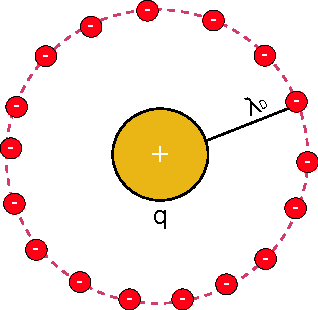
\includegraphics[width = 0.4\textwidth]{Figures/Cap 2/elek_Layer 1.pdf}
        \caption{Representation of the ion being sorrounded by an electronic cloud with spherical symmetry.}
        \label{fig:SpheSym}
    \end{figure}

    We can see in the equation \ref{eq:ShieldPot} that the potential decays faster than a Coulombian potential, this is due to the presence of the charges surrounding the ions, because they have, most of times, opposite charge the net interaction becomes diminished, this is called a shielding we can represent it like in the figure \ref{fig:CVsShield}. Now lets give a look to the potential difference

    \begin{figure}[h]
        \centering
        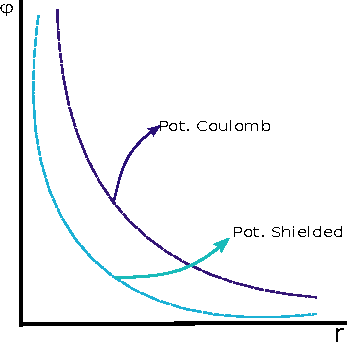
\includegraphics[width = 0.3\textwidth]{Figures/Cap 2/aroo_Layer 1.pdf}
        \caption{Graph comparision between the coulombian potential an the shielded potential.}
        \label{fig:CVsShield}
    \end{figure}

    \begin{equation}
        \triangle \phi = \phi_D - \phi_C = \frac{q}{4\pi\epsilon_0r}(e^{-r/\lambda_D} - 1)\;
    \end{equation}

    If $r \ll \lambda_D$ we gave got:
    \begin{equation}
        \triangle\phi = -\frac{q}{4\pi\epsilon_0\lambda_D}
    \end{equation}

    This is the potential generated by the surrounding charged around the nucleus as is shown in \ref{fig:SpheSym}. Now lets give a look to the total energy of the system, taking the energy as the work needed from moving a charge from the infinity a bringing it to their position is:

    \begin{equation}
        W = -\frac{1}{8\pi\epsilon_0}\sum_s\frac{e_s^2}{\lambda_D}\;\;:\;\; s=i,e
    \end{equation}

    \begin{equation*}
        W = -\frac{1}{8\pi\epsilon_0}\sum_s\frac{e_s^2}{\lambda_D^3}\lambda_D^2
    \end{equation*}

    \begin{equation*}
        W_e = -\frac{e^2}{8\pi\epsilon_0\lambda_D^3}\left(\frac{\epsilon_0K_B\Bar{T}}{n_0e^2}\right) = -\frac{K_B\Bar{T}}{8\pi\epsilon_0\lambda_D^3n_0}
    \end{equation*}

    We can now define the \textbf{plasma number} $\Lambda_D$ as: $\N_D = \frac{4}{3}\pi\lambda_D^3n_0 = \frac{\Lambda_D}{3}$ thus:

    \begin{equation}
        W_e = -\frac{K_B\Bar{T}}{6N_d}
    \end{equation}

    \begin{itemize}
        \item $W_e \ll K_BT$ we have got a few collisional plasma, this is because the electron energy is less than the average kinetic energy and this implies $N_d \gg 1$

        \item $W_e \gg K_BT$ the plasma is really collisional, this implies the electrons energy is bigger than the average kinetic energy and also implies $N_d \ll 1$.
        
    \end{itemize}

    \subsection{Plasma parameters}
        The following parameters characterize the plasma:
        \begin{enumerate}
            \item The plasma natural frequency $\omega_p$.
            \item The Debye's length or the Debye's shielding length $\lambda_D$.
            \item The plasma number $N_D(\Lambda_D)$
        \end{enumerate}

        With this we can now give a new definition from plasma as follows: \textbf{The plasma is a quasi-neutral gas $(L \gg \lambda_D$) of charged, and neutral particles, which shows collective behaviors.}

    \section{Collisions a macroscopic vision}

        Here a really important concept is gonna be developed the concept of collision in a classical sense to do this some concepts are going to appear:

        \begin{itemize}
            \item \textbf{Forces among charged particles:} This particles are going to interact by Coulomb forces , those are long distance interactions.

            \item \textbf{Forces among the particles in a plasma:} Here the Coulomb forces are going to be shielded by a Debye's shielding, but how much do these forces variate? That depend on the collision frequency.

            \item \textbf{Collisions frequency:} Is a scattering whose effect is changing the momentum of the charged particles.
        \end{itemize}

        \subsection{Collisions frequency}
            \begin{figure}[h]
                \centering
                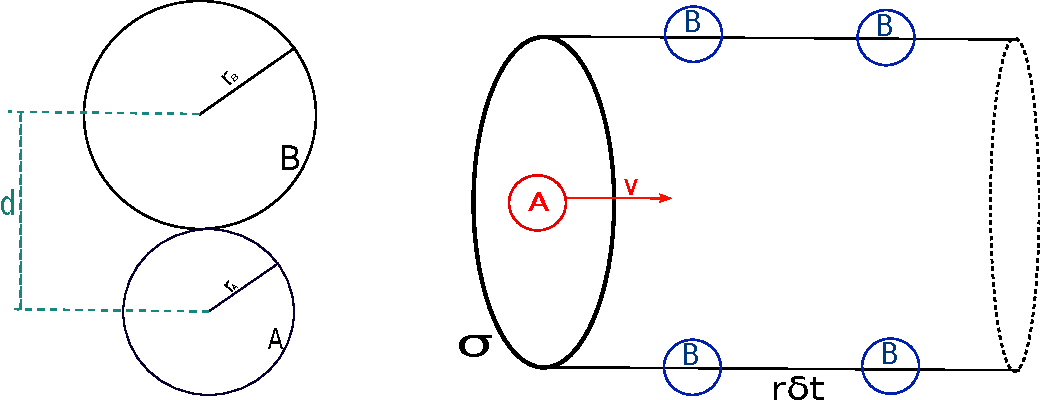
\includegraphics[width = 0.8\textwidth]{Figures/cap 3/ara_Layer 1.pdf}
                \caption{Representation of two atoms an the interaction distance D, also in the right there is an illustration of the effective volume of interaction of the particles A and B.}
                \label{fig:ara}
            \end{figure}

            From the kinetic theory there is a time of  collisions as follows:

            \begin{equation}
                \tau_c = \frac{1}{n\mathbf{v}\sigma}
            \end{equation}

            Where $\sigma$ is an effective collisions area . We talk about collisions where there are an exchange of momentum and not only that because also exchange internal energy. There are elastic and inelastic collisions as in the ionization.

            In the figure \ref{fig:ara} there is a graphical representation of our particles and the effective volume, here there are at least two species of particles, all are going to be represented as classical particles of radius $r_B$ and $r_B$ this radius represents a solid distance but represents the mininal distance of interactin from the particle, thus the effective distance is the sum of both radius $d = r_B + r_A$.\\

            Let $N_A$ and $N_B$ the number of particles in the volume then:

            \begin{equation*}
                n_a = \frac{N_A}{V} \;\;\; n_b = \frac{N_B}{V}
            \end{equation*}

            So lets define an effective are where there is gonna be a collision:

            \begin{equation}
                \sigma = \pi(r_A + r_B)^2 = \pi d^2
            \end{equation}

            \begin{equation}
                V = \mathbf{v} \triangle t \sigma
            \end{equation}

            \begin{equation*}
                N_B = \mathbf{v}\triangle t \sigma \frac{N_B}{V} \rightarrow \frac{N_B}{\triangle t} = \mathbf{v}\sigma n_B
            \end{equation*}

            As we can see there is a new term that shows how many $B$ particles interact per time thus we can define a collisions frequency for $B$:

            \begin{equation}
                \nu_c = \mathbf{v}\sigma n_B
            \end{equation}

            Now, instead of thinking on rigid spheres lets thinks about columb interactions, so the movement of the particles looks like in the figure \ref{fig:uy}

            \begin{equation}
                \tau_c = \frac{1}{\mu_c} = \frac{1}{\mathbf{v}\sigma n_B}
            \end{equation}

            \begin{figure}[h]
                \centering
                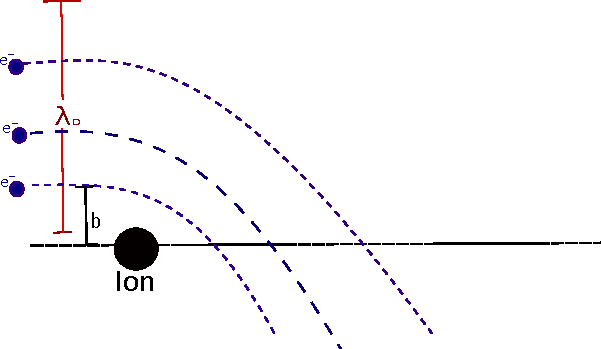
\includegraphics{Figures/cap 3/uy_Layer 1_copy_2.pdf}
                \caption{Representation of the columb interaction in the plasma.}
                \label{fig:uy}
        \end{figure}

        The value $b$ is also known as the critic radius so to calculate it we must have a balance of energy, this means $U = K$:

        \begin{equation*}
            \frac{ze^2}{4\pi\epsilon_0b} = \frac{m_av_A^2}{2}
        \end{equation*}

        \begin{equation}
            b = \frac{2ze^2}{4\pi\epsilon_0m_Av_A^2}
        \end{equation}

        In this case $N_A = N_e$ and $N_B = N_i$ the number of electrons and ions, respectively, and the effective area is $\sigma = \pi b^2$.

        \begin{equation*}
            \nu_c = n_B\sigma v_A = n_Bv_A\pi b^2
        \end{equation*}

        \begin{equation}
            \nu_c = \frac{z^2e^4n_B}{4\pi\epsilon_0^2m_A^2v_A^3}
        \end{equation}

        Suppose we have a plasma of ions and electrons, then exists a collisions frequency $\nu^c_{i,e}$:

        \begin{equation}
            \nu_{ie}^c = \frac{z^2e^4n_i}{4\pi\epsilon_0^2m_e^2v_e^3}\;\;v_e = \sqrt{\frac{K_BT_e}{m_e}}
        \end{equation}

        So there are a collisions frequency and a natural frequency, both can be compared, thus:

        \begin{equation}
            \nu_{ie}^c = \frac{z^2e^4n_i}{4\pi\epsilon_0^2m_e^{1/2}}(K_BT)^{-3/2}
        \end{equation}

        \begin{equation}
            \omega_p^2 = \frac{n_ee^2}{\epsilon_0m_e}
        \end{equation}


        \begin{equation}
            \nu_{ie}^c = \frac{z^2e^4n_i}{4\pi\epsilon_0^{3/2}n_e}\omega_p(K_BT)^{-3/2}
        \end{equation}

        And we can see that the last expression can be related to a Debye's length and Debye's plasma number: 

        \begin{equation}
            \lambda_D = \frac{\epsilon_0K_BT}{n_ee^2}
        \end{equation}

        \begin{equation}
            \Lambda = 4\pi n \lambda_D^3
        \end{equation}

        \begin{equation}
            \frac{\nu_{ie}}{\omega_p} = \frac{z^2n_i}{4\pi n_e^2}\frac{1}{\lambda_D^3}
        \end{equation}

        Because the plasma is globally neutral $n_e \approx n_i = n$.
        
        \begin{equation}\label{eq:frequencies}
            \frac{\nu_{ie}^c}{\omega_p} = \frac{z^2}{\Lambda}
        \end{equation}

        \begin{enumerate}
            \item $\Lambda \gg 1$ The system is weakly bounded this means a plasma with few collisions $\nu^c_{ie} \ll \omega_p$ this implies that \textit{the collisions times are bigger than the Debye's times.}

            \item $\Lambda \ll 1$ this is a plasma with lot of collisions  and $\nu^c_{ie} \gg \omega_p$ here the collisions become relevant to the system dynamics, this plasma can be studied with the \textit{approximation of the magnetohydrodinamics}.
        \end{enumerate}

        It becomes necessary to correct this formula because not only there is the contribution of an individual electron, an ion has an excess of charge then in an \textbf{empirical way} the formula is: 

        \begin{equation}\label{eq:}
            \frac{\nu^c_{ie}}{\omega_p} \approx \frac{Ln(\Lambda)}{\Lambda}
        \end{equation}

        \begin{equation*}
            Ln(\Lambda) = Ln(\frac{2\lambda_D}{b}) \approx 15 ~ 20
        \end{equation*}


    \section{Particles movement in magnetic fields}

        In the electromagnetism we have the so called Lorentz's force:

        \begin{equation}
            m\frac{d\Vec{U}}{dt} = q(\Vec{E} + \Vec{U}\times \Vec{B})
        \end{equation}

        Let suppose a magnetic field constant in magnitude and direction, also there is no electric field, thus: $\Vec{B} = B_0\hat{e}_z$

        \begin{equation*}
            m\frac{dU_x}{dt}=qU_yB_0
        \end{equation*}

        \begin{equation*}
            m\frac{dU_y}{dt}=qU_xB_0
        \end{equation*}

        \begin{equation*}
            m\frac{dU_z}{dt} = 0 \rightarrow U_z = cte
        \end{equation*}

        We  can rewrite that system of equations in the following way:

        \begin{equation*}
            U = U_x + iU_y \rightarrow m\frac{dU}{dt} = -iqBU
        \end{equation*}

        This equation ins easilly to solve:

        \begin{equation}
            U = U_0e^{-iqBt/m}
        \end{equation}

        \begin{equation}
            \Vec{U_0}= [0,U_{0y},U_{0z}] \;\;Initial\;\;condition.
        \end{equation}

        \begin{equation*}
            U = U_{0y}sin\left(\frac{qBt}{m} \right) + iU_{0y}cos\left(\frac{qB}{m}t\right)
        \end{equation*}

        Thus, we have the following trayectories:

        \begin{equation}\label{eq:mvx}
            x = x_0 - \frac{U_{0y}m}{qB}cos\left(\frac{qB}{m}t\right)
        \end{equation}

        \begin{equation}\label{eq:mvy}
            x = y_0 + \frac{U_{0y}m}{qB}sin\left(\frac{qB}{m}t\right)
        \end{equation}

        \begin{equation}
            z = z_0 + U_{0z}t
        \end{equation}

        This is a helicoidal trajectory centered in $(x_0,y_0)$ which radius is the Lamor's radius, this decribes the radius of a particle inside a uniform magnetic field:

        \begin{equation}\label{eq:LarmorRad}
            r = \frac{U_{\perp}m}{|qB|}
        \end{equation}

        In a generic way: $U_{\perp} = \sqrt{U_x^2 + U_y^2}$ here we can also define a frequency, the so called cyclotron frequency $\omega_i = \frac{|q|B}{m}$.

        \subsection{Drift of particles in electromagnetic fields}

            Here we are going to consider a non relativistic version of the drift velocity so lets start with a kind of generalized version of the Lorent'z force where we're going to consider an arbitrary force $\Vec{F}$:

            \begin{equation}
                m\frac{d\Vec{U}}{dt} = \Vec{F} + q\Vec{U}\times\Vec{B}
            \end{equation}

            Now, were goint to step on an intertial reference system $\mathcal{O}'$ which moves with constant speed $\Vec{V}_D$ thus the addition of speed rule gives us:

            \begin{equation*}
                \Vec{U}' = \Vec{U} - \Vec{V}_D
            \end{equation*}

            \begin{equation}
                m\frac{d\Vec{U}}{dt} = \Vec{F} + q(\Vec{U}' + \Vec{V}_D)\times\Vec{B}
            \end{equation}

            We can choose an equation such that $\Vec{F} + q\Vec{V}_D\times\Vec{B} = 0$ this means we choose a drift speed such that in that reference frame the total force is:

            \begin{equation}
                m\frac{d\Vec{U}'}{dt} = q\Vec{U}'\times\Vec{B}
            \end{equation}

            The main idea is to find a reference frame such that there the trajectory would be the equation solved before, in this way $\Vec{V}_D$ appears not only for an electric field but to ta general force $\Vec{F}$

            \begin{equation}
                \Vec{B}\times\Vec{F} + q\Vec{B}\times\Vec{V}_D\times\Vec{B} = 0
            \end{equation}

            \begin{equation*}
                \Vec{B}\times\Vec{F} + q[\Vec{V}_DB^2 - \Vec{B}(\Vec{B}\cdot\Vec{V}_D)] = 0
            \end{equation*}

            We can decompose $\Vec{V}_D$ as $\Vec{V}_D = \Vec{V}_{D\paralell} + \Vec{V}_{D\perp}$ thus:

            \begin{equation}
                \Vec{V}_{D\perp} = \frac{\Vec{F}_{\perp}\times\Vec{B}}{qB^2} \;\;\&\;\; \Vec{V}_{D\paralell} = 0
            \end{equation}

            In general $\Vec{V}_D$ is not constant thus:

            \begin{equation}
                m\frac{d\Vec{U}'}{dt} = \Vec{F} - m\frac{d\Vec{V}_d}{dt} + q(\Vec{U}' + \Vec{V}_D)\times\Vec{B}
            \end{equation}

            \begin{equation*}
                \Vec{F} - m\frac{d\Vec{V}_D}{dt} + q\Vec{V}_D\times\Vec{B} = 0 \rightarrow m\frac{d\Vec{U}'}{dt} = q\Vec{U}'\times\Vec{B}
            \end{equation*}

            \begin{equation}
                \Vec{B}\times\Vec{F} - m\Vec{B}\times\frac{d\Vec{V}_d}{dt} + q[\Vec{V}_DB^2 - \Vec{B}(\Vec{V}_D\cdot\Vec{B})]=0
            \end{equation}

            \begin{equation*}
                \Vec{B}\times\Vec{F}_{\perp} - m\Vec{B}\times\frac{d\Vec{V}_{D\perp}}{dt} + q \Vec{V}_{D\perp}B^2 = 0
            \end{equation*}

            \begin{equation}
                \Vec{V}_{D\perp} = \frac{1}{qB^2}\left[\Vec{F}_{\perp} - m\frac{d\Vec{V}_{D\perp}}{dt}\right]\times\Vec{B}
            \end{equation}

            \begin{equation}
                \Vec{F}_{\parallel} = m\frac{d\Vec{V}_{D\parallel}}{d}
            \end{equation}

        \subsection{Example and relation between $E$ and $B$}

            Let $\Vec{F} = q\Vec{E}$ a coulombian force and the drift speed constant $\Vec{V}_D = cte$ thus:

            \begin{equation}\label{eq:VDperp}
                \Vec{V}_{D\perp} = \frac{\Vec{E}_l \times\Vec{B}}{B^2}
            \end{equation}

            And because we known $\Vec{U}'$ and we've got the equation for $\Vec{V}_D$ we can find $\Vec{U}$:

            \begin{equation}
                \Vec{U} = \Vec{U}' + \Vec{V}_{D\perp} + \Vec{V}_{D\parallel}
            \end{equation}

            Now there are two casses:

            \begin{enumerate}
                \item $||\Vec{E}_{\perp}|| \ll ||\Vec{B}|| $ the non relativistic domain.

                \item$||\Vec{E}_{\perp}|| \gg ||\Vec{B}|| $ the relativistic domain.
            \end{enumerate}

            From the Amepere's law and Faraday's law we have got:

            \begin{equation}
                \frac{1}{C^2}\frac{\partial\Vec{E}}{\partial t} \approx \frac{1}{C^2}\frac{E_0}{t_0^2} \approx \frac{V_0}{C^2}\frac{E_0}{l_0}
            \end{equation}

            \begin{equation}
                \frac{E_0}{l_0}\approx \frac{B_0}{t_0}\approx \frac{V_0}{l_0}B_0 \approx V_0|\Vec{\nabla}\times\Vec{B}|
            \end{equation}

            In general the most important thing is the relation between the circulation of the magnetic field and the displacement currents, in fact, in the non relativistic realm we have

            \begin{equation}
                |\Vec{\nabla}\times\Vec{B}| \gg \frac{1}{C^2}\left|\frac{\partial\Vec{E}}{\partial t} \right|
            \end{equation}

    \section{Drift movements in non uniform stationary magnetic fields}

        From here on we want to make the use of the theory of perturbations. The magnetic field now is going to have a small perturbation this means it will be lightly different from the original to do that mathematically we make an expansion of the magnetic field and cut it off at the first order, also for our mathematical development the magnetic field is parallel to $\hat{e}_z$ thus:

        \begin{equation}
            m\frac{d\Vec{U}_{\perp}}{dt} = q\Vec{U}_{\perp}\times\left[\Vec{B}_0 + (x-x_0)\frac{\partial\Vec{B}}{\partial x}|_{x_0} + (y-y_0)\frac{\partial\Vec{B}}{\partial y}|_{y_0} \right]
        \end{equation}

        The axis of the helix is at $(x_0,y_0)$ where teh field is $\Vec{B}_0$ and we can find the difference $(x-x_0)$ and $(y-y_0)$ from the equations \ref{eq:mvx} and \ref{eq:mvy} respectively thus we have:

        \begin{equation*}
            \Vec{U}_{\perp} = U_x\hat{e}_x + U_y\hat{e}_y \;\;and\;\; \Vec{B} = B(x,y)\hat{e}_z
        \end{equation*}

        \begin{equation*}
            \Vec{F}_{\perp} = qU_x(x-x_0)\frac{\partial B}{\partial x}(-\hat{e}_y) + qU_y(x-x_0)\frac{\partial B}{\partial x}\hat{e}_x + qU_x(y-y_0)\frac{\partial B}{\partial y}(-\hat{e}_y) + qU_y(y-y_0)\frac{\partial B}{\partial y}\hat{e}_x
        \end{equation*}

        \begin{equation*}
            \Vec{F}_{\perp} = qU_{y0}^2sin\left(\frac{qB}{m}t \right)\frac{m}{qB}cos\left(\frac{qB}{m}t \right)\frac{\partial B}{\partial x}|_{x0}\hat{e}_y + qu_{y0}^2cos\left(\frac{qB}{m}t \right)\frac{mq}{B}cos\left(\frac{qB}{m}t \right)\frac{\partial B}{\partial x}(-\hat{e}_x) + ...
        \end{equation*}

        Now we want to analyze the system at a time greater than the cyclotron ($t \gg \frac{2\pi}{\omega_c}$) time that is because we want to analyze the behavior of the system while this evolves, to analyze this average time must be taken, young Padawan:

        \begin{equation}
            <...> = \frac{1}{T_c}\int_t^{t + \tau_c}(...)dt\;.
        \end{equation}

        Thus,

        \begin{equation}
            <\Vec{F}_{\perp}> = -\frac{1}{2}U_{\perp}^2\frac{m}{B}\Vec{\nabla}_{\perp}B \;\;,
        \end{equation}

        and using the Larmor's radius \ref{eq:LarmorRad}:

        \begin{equation}
            <\Vec{F}_{\perp}> = -\frac{1}{2}|q|r_{\perp}^2\omega_c\Vec{\nabla}_{\perp}B
        \end{equation}

        We can see that the time average of the perpendicular force looks like a centripetal force where the charge plays the role of the inertia the Larmor's radius and the cyclotron frequency play the role of the tangential speed and the perpendicular gradient of $B$ give the direction of this acceleration. Now, solving for the perpendicular component of the  drift speed:
        
        \begin{equation*}
            \Vec{V}_{D\perp}= \frac{\Vec{F}_{\perp} \times \Vec{B}}{|q|B^2}= -\frac{1}{2}|q|r_{\perp}^2\omega_c \frac{\Vec{\nabla}_{\perp}B \times \Vec{B}}{|q|B^2} = \frac{1}{2}mU_{\perp}^2 \frac{\Vec{\nabla}_{\perp} \times \Vec{B}}{|q|B^2}
        \end{equation*} 

        \begin{equation}
            \Vec{V}_{D\perp} = - K_{\perp}\frac{\Vec{\nabla}_{\perp}B \times \Vec{B}}{|q| B^3}\;\;,
        \end{equation}

        \subsection{Magnetic field $\Vec{B}$ with constant magnitude but with a light curve}

            \begin{figure}[h]
                \centering
                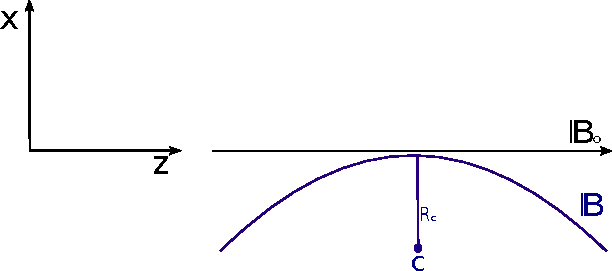
\includegraphics[width = 0.8\textwidth]{Figures/Cap 4/FirstDev.pdf}
                \caption{Initial magnetic field $\Vec{B}_0$ compared with the new (curved) magnetic field $\Vec{B}$.}
                \label{fig:CurvedB}
            \end{figure}

            Again we're going to use perturbation theory, thus the Lorentz's force equation in a reference system where there's only magnetic field becomes:

            \begin{equation}
                m\frac{d\Vec{U}}{dt} = q\Vec{U}\times\Vec{B} \approx q\Vec{U} \times \left[\Vec{B}_0 + (z-z_0)\frac{\partial B_x}{\partial z}|_0 \hat{e}_x \right]\;,
            \end{equation}

            \begin{equation*}
                m\frac{d\Vec{U}}{dt} \approx q\Vec{U}\times\Vec{B}_0 + q\Vec{U}\times(z-z_0)\partial_zB_x|_0\hat{e}_x\;\;and\;\; U_z = U_x = cte \rightarrow z = z_0 + U_{\parallel}t\;\;.
            \end{equation*}

            Now, for the perpendicular component of the force:

            \begin{equation*}
                \Vec{F}_{\perp} = qU_{\parallel}\hat{e}_x \times (z-z_0)\partial_zB_x|_0\hat{e}_x\;\;,
            \end{equation*}

            \begin{equation*}
                \Vec{F}_{\perp} = qU_{\parallel}(z-z_0)\partial_zB_x|_0\hat{e_y}\;\;,
            \end{equation*}

            \begin{equation*}
                \Vec{F}_{\perp} = qU_{\parallel}^2t\partial_zB_x|_0\hat{e}_y\;\;.
            \end{equation*}

            Now, analyzing the curve we have got a direct relation with $\partial_zB_x|_0$ in the following way:

            \begin{equation}
                \partial_zB_x|_0 = -\frac{B_0}{R_c}
            \end{equation}

            This relation is strictly related to the fact that in a curve $\Vec{\tau}$ with a parameter $s$  there is a direct relation with the curvature radius as $\frac{d \Vec{\tau}}{d s} = \frac{1}{R_c}\hat{n}$ thus the perpendicular component of the force becomes:

            \begin{equation}
                \Vec{F}_{\perp} = -qU_{\parallel}^2t\frac{B_0}{R_c}\hat{e}_y\;.
            \end{equation}

            Lets generalize it for a magnetic field more curved, if we look at carefully the figure \ref{fig:CurvedB} we can see that the vectors $\Vec{B}_0$ and $\Vec{R}_0$ set the direction of the perpendicular force, because they're orthogonal and their cross product can define us the direction of the perpendicular force, thus:

            \begin{equation}\label{eq:CovFPerp}
                \Vec{F}_{\perp} = qU_{\parallel}^2t\frac{\Vec{R}_c \times \Vec{B}}{R_c^2}\;\;.
            \end{equation}

            The equation \ref{eq:CovFPerp} represents a covariant form of the perpendicular force, in this way the movement equation becomes:

            \begin{equation}
                m\frac{d\Vec{U}}{dt} = q\Vec{U}\times\Vec{B} + qU_{\parallel}^2t\frac{\Vec{R}_c \times \Vec{B}}{R_c^2}\;.
            \end{equation}

            We're going to analyze the analytical solution of this problem but using an arbitrary observer $\mathcal{O}$ where the drift speed $\Vec{V}_D$ is perpendicular to the field and the parallel compoments are equal $U_{\parallel} = U'_{\parallel}$ thus:

            \begin{equation*}
                m\frac{d\Vec{U'}}{dt} + m\frac{d\Vec{V}_D}{dt} = q(\Vec{U'} + \Vec{V}_D) \times \Vec{B} + qU_{\parallel}^2t\frac{\Vec{R_c}\times \Vec{B}}{R_c^2}\;,
            \end{equation*}

            \begin{equation*}
                m\frac{d\Vec{U'}}{dt} = q(\Vec{U'} + \Vec{V}_D)\times\Vec{B} + qU_{\parallel}^2t\frac{\Vec{R}_c \times \Vec{B}}{R_c^2} - m\frac{d\Vec{V}_D}{dt}\;.
            \end{equation*}

            We're going to decompose the drift velocity as $\Vec{V}_D = \Vec{V}_{D1} + \Vec{V}_{D2}:$

            \begin{equation*}
                m\frac{d\Vec{U'}}{dt} = q(\Vec{U'} + \Vec{V}_{D1}) \times \Vec{B} + qU_{\parallel}^2t\frac{\Vec{R_c}\times\Vec{B}}{R_c^2}\;,
            \end{equation*}

            By analogy with the case of $\Vec{V}_D$ constant we have got:

            \begin{equation}
                \Vec{V}_{D1} = -U_{\parallel}^2t\frac{\Vec{R_c}\times \Vec{B}}{B^2R_c^2}\times \Vec{B} = -U_{\parallel}^2t\frac{\Vec{R}_c}{R_c^2}\;.
            \end{equation}

            Now with this solution for the first component we can solve the general problem as follows:

            \begin{equation*}
                m\frac{d\Vec{U'}}{dt} = q(\Vec{U'} + \Vec{V}_{D1} + \Vec{V}_{D2})\times\Vec{B} + qU_{\parallel}^2t \frac{\Vec{R}_c\times\Vec{B}}{R_c^2} - m\frac{d}{dt}(\Vec{V}_{D1} + \Vec{V}_{D2})\;,
            \end{equation*}

            \begin{equation}
                m\frac{d\Vec{U'}}{dt} = q(\Vec{U'} + \Vec{V}_{D2})\times \Vec{B} + mU_{\parallel}^2\frac{\Vec{R}_c}{R_c^2} - m\frac{d\Vec{V}_{D2}}{dt}\;.
            \end{equation}

            $\Vec{V}_{D1}$ is not constant but for the second component we  can suppose it constant why? because yes, this is a mathematical tool that is useful. 

            \begin{equation}
                \Vec{V}_{D2} = \frac{mU^2_{\parallel}}{q}\frac{\Vec{R}_c \times \Vec{B}}{R_c^2B^2}\;,
            \end{equation}

            \begin{equation}
                \Vec{V}_D = -U_{\parallel}^2t\frac{\Vec{R}_c}{R_c^2} + \frac{mU_{\parallel}^2}{q}\frac{\Vec{R}_c \times \Vec{B}}{R_c^2 B^2}\;.
            \end{equation}

            In a reference frame with speed $\Vec{V}_D$ the Lorentz's force become the well known equation for the helical motion. 

        \subsection{$\Vec{B}$ parallel to the x-axis with a variation along the z-axis}

        \begin{figure}[h]
            \centering
            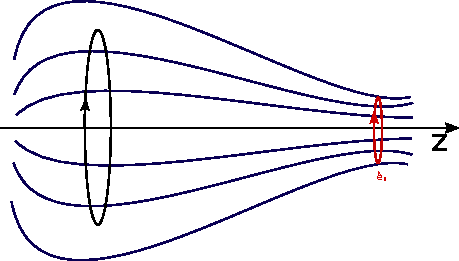
\includegraphics[width = 0.8\textwidth]{Figures/Cap 4/Tube.pdf}
            \caption{Magnetic field with a bottle like behavior, this magnetic fields are used to confine plasma using a mirror effect in the zone where it stretches.}
            \label{fig:tubeMag}
        \end{figure}

        Here we're going to use cylindrical coordinates and a magnetic field such that:

        \begin{equation}
            \Vec{B} = [B_r,0,B_z]\;\;|\;\; \partial_{\theta}\Vec{B} = 0
        \end{equation}

        Now from the Gauss's law is easy to see:

        \begin{equation*}
            \Vec{\nabla}\cdot\Vec{B} = 0 \rightarrow \partial_zB_z = -\frac{1}{r}\partial_r(rB_r)\;,
        \end{equation*}

        We want to find a relation between the radial and the z components of the magnetic field, to do that we can take the angular average $<...>_{\theta}$ of the last equation:

        \begin{equation*}
            r<B_r>_{\theta} = -\frac{r^2}{2}\partial_z<B_z>_{\theta} \rightarrow <B_r> = -\frac{r}{2}\partial_z<B_z>_{\theta}\;,
        \end{equation*}

        \begin{equation*}
            \partial_z<B_z>_{\theta} = -\frac{1}{r}\partial_r(r<B_r>_{\theta}) = -\partial_r<B_r>_{\theta} - \frac{1}{r}<B_r>_{\theta} = -2\frac{<B_r>}{r}\;,
        \end{equation*}

        the force is given by:

        \begin{equation}
            \Vec{F} = q\Vec{U}_{\perp}\times<B_r>\hat{e}_r
        \end{equation}

        \textbf{Demonstration:} METER ACÁ LA DEMOSTRASAO

        So the force now becomes:

        \begin{equation}
            \Vec{F} = -q\Vec{U}_{\perp}\times \frac{r}{2}\partial_z<B_z>\hat{e}_r = -\frac{mU_{\perp}^2}{2B}\partial_z<B_z>\hat{e}_z
        \end{equation}

        \begin{figure}[h]
            \centering
            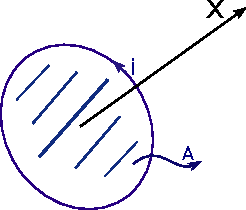
\includegraphics[width = 0.4\textwidth]{Figures/Cap 4/Dipole.pdf}
            \caption{Illustration of the dipole magnetic moment for a current loop which encloses an area $A$.}
            \label{fig:DipoleExam}
        \end{figure}

        Here we can identify the magnetic moment which defines not only the magnitude of the magnetic field and the orientability of the material. It is given by:

        \begin{equation}
            \mu = \frac{1}{2}m\frac{U_{\perp}^2}{B}\;.
        \end{equation}

        From the figure \ref{fig:DipoleExam} we can deduce the last expression:

        \begin{equation}
            \mu = iA \;\; |\;\; i = \frac{|q|}{\tau} \;\; \tau = \frac{2\pi}{\omega_c} \;\; A = \pi r_L^2\;,
        \end{equation}

        \begin{equation}
            \mu = \frac{|q|\omega_c\pi r_L^2}{2\pi} = \frac{1}{2}\frac{mU_{\perp}^2}{B}\;.
        \end{equation}

        Generalizing we have then: 

        \begin{equation}
            \Vec{F}_{\parallel} = -\mu \Vec{\nabla}B\;.
        \end{equation}

        But how is the evolution of $\mu$ respect to the other variables? To answer this we must analyze the conservation of the kinetic energy because in our system there is no reason our energy doesn't conserve, in this way we have got:

        \begin{equation*}
            \frac{dW_{\parallel}}{dt}=\frac{m}{2}\frac{dU_{\parallel}^2}{dt}=mU_{\parallel}\frac{dU_{\parallel}}{dt}
        \end{equation*}

        \begin{equation*}
            \frac{dW_{\parallel}}{dt} = -\frac{W_{\perp}}{B}\partial_zB_zU_{\parallel} = -\frac{W_{\perp}}{B}\frac{dB}{dt}
        \end{equation*}

        We can see that the conservation of the energy depend on the magnetic field, if this depends or not of time, thus:

        \begin{equation*}
            W = W_{\perp} + W_{\parallel} = cte \rightarrow \frac{dW}{dt} = \frac{dW_{\parallel}}{dt} + \frac{dW_{\perp}}{dt} = 0\rightarrow \frac{dW_{\perp}}{dt} = \frac{W_{\perp}}{B}\frac{dB}{dt}\;
        \end{equation*}

        This implies that the magnetic moment ins constant and invariant. If $\mu$ is invariante the parallel force depends on the gradiente of $B$ if this gradiente is big enough there will be a effect of a mirror, because the force will go to the left and the particle will be reflected, but this not always happen because there is a certain angle respect to the z-axis where the particle can cross the magnetic field and won't be reflected, lets calculate that angle.

    \section{Adiabatic invariants}

    Lets talk about slow changes in a closed trajectory. The main idea of this is to relate the energy with the frequency and this is what we call an adiabatic invariant.
    An adiabatic invariant is a physical quantity that remains constant during an adiabatic process. An adiabatic process is one in which there is no heat transfer between the system and its surroundings. This means that the internal energy of the system remains constant throughout the process.\\

    A common example of an adiabatic invariant is entropy. During an adiabatic process, the entropy of the system remains constant, which means there is no change in the amount of disorder or randomness in the system.\\

    Another example of an adiabatic invariant is angular momentum in quantum mechanics. During an adiabatic process, the angular momentum of the system remains constant. This is because angular momentum is a conserved quantity in an isolated system in which there are no external forces acting on the system.\\

    In general, adiabatic invariants are useful for describing and understanding the conservation of certain physical quantities during processes in which there is no heat transfer.\\

    Lets consider a physical system in generalyzed coordinates which changes with a parameters $\lambda$. The movements bounded by $V(q)$ can be periodic.

    \begin{figure}[h]
        \centering
        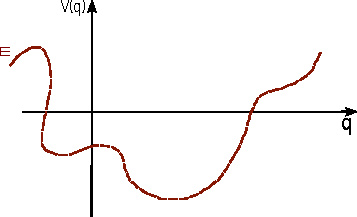
\includegraphics[width = 0.7\textwidth]{Figures/Cap 5/trajectory.pdf}
        \caption{Example of the potential energy function $V(q)$ which varies with $q$.}
        \label{fig:trajectory}
    \end{figure}

    Do the trajectory changes adiabatically? Lets think about in a harmonic oscillator whose energy starts to change slowly:

    \begin{equation}
        \Dot{E} = \frac{\partial H}{\partial \lambda}\Dot{\lambda}
    \end{equation}

    Are there combinations of $E$ and $\lambda$ such that the energy of the system keeps constant? For example, lets consider the following hamiltonian:

    \begin{equation*}
        H = \frac{p^2}{2m} + V(q,\lambda(t)) = H(q,p,\lambda(t)) \;\;and\;\; \frac{\partial H}{\partial t} = \Dot{\lambda}\frac{\partial H}{\partial \lambda}\;.
    \end{equation*}

    We're going to analye the temporal average of the physical system such that $\Dot{\lambda} = cte$:

    \begin{equation}
        <\frac{\partial H}{\partial t}> = \Dot{\lambda}<\frac{\partial H}{\partial \lambda}> = \frac{\Dot{\lambda}}{T}\int_0^T\frac{\partial H}{\partial \lambda}dt
    \end{equation}

    Now, from the Hamilton's equations we've got:

    \begin{equation}
        \frac{\partial H}{\partial p} = \frac{dq}{dt}\;,
    \end{equation}

    Thus:

    \begin{equation*}
        dt = \left(\frac{\partial H}{\partial p} \right)^{-1}dq \;\;and\;\; T = \int_0^Tdt
    \end{equation*}

    \begin{equation}
        <\frac{\partial H}{\partial t}>\oint \left(\frac{\partial H}{\partial p}\right)^{-1}dq = \Dot{\lambda}\oint \frac{\partial H}{\partial \lambda}\left(\frac{\partial H}{\partial p}\right)^{-1}dq
    \end{equation}

    \begin{equation}
        \oint \left[<\frac{\partial H}{\partial t}> \frac{\partial p}{\partial H} - \Dot{\lambda}\frac{\partial H}{\partial \lambda}\left(\frac{\partial H}{\partial p} \right)^{-1} \right]dq = 0
    \end{equation}

    Now, because we want the energy to change smoothly with $\lambda$ then $dH = 0$, then we have:

    \begin{equation}\label{eq:dHLmd}
        \frac{dH}{d\lambda} = \frac{\partial H}{\partial q}\frac{\partial q}{\partial \lambda} + \frac{\partial H}{\partial P }\frac{\partial p}{\partial \lambda} + \frac{\partial H}{\partial \lambda} \approx 0
    \end{equation}

    Lets keep two variables constant respect to the parameter $\label{}$, in our case those are going to be the energy an the generalized position, then from the equation \ref{eq:dHLmd}:

    \begin{equation}
        \frac{\partial H}{\partial \lambda} \approx - \frac{\partial H}{\partial p} \frac{\partial p}{\partial \lambda}
    \end{equation}

    So we have the following equation:

    \begin{equation}
        \oint \left[<\frac{\partial H}{\partial t}>\frac{\partial p}{\partial H} + \Dot{\lambda}\frac{\partial p}{\partial \lambda} \right]dq = 0
    \end{equation}

    If we look carefully that closed integral can be expressed as an exact differential as follows:

    \begin{equation}
        \frac{d}{dt}<\oint pdq> = 0
    \end{equation}

    We can see there is a conservation law from this, we define an action variable, an \textbf{adiabatic invariant} $J$ which is related to the Sommerfeld's quantization rule \ref{APX:Sommerfeld}:

    \begin{equation}
        J = \frac{1}{2\pi}\oint pdq = cte
    \end{equation}

    Now, lets think about in the following invariant $J$:

    \begin{equation}\label{eq:InvAdiaba}
        J = \frac{1}{2\pi}\oint_{c(t)}\Vec{p}\cdot \Vec{dq}
    \end{equation}

    So, to think about the movement of a charged particle under the effect of a magnetic field, we can use Lagrangian mechanics, so the Lagrangian is the following:

    \begin{equation}
        \mathcal{L} = \frac{1}{2}mv^2 + e \Vec{r}\cdot\Vec{A} \;,
    \end{equation}

    \begin{equation}
        \Vec{P} = \frac{\partial \mathcal{L}}{\partial \Vec{v}} = m\Vec{v} +e \Vec{A}\;.
    \end{equation}

    \begin{figure}[h]
        \centering
        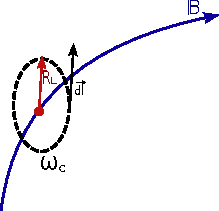
\includegraphics[width = 0.5\textwidth]{Figures/Cap 5/BField.pdf}
        \caption{Magnetic field and the relation among the path differential, $\Vec{dl}$ Larmor's radius $R_L$ and the cyclotron frequency $\omega_c$.}
        \label{fig:BField}
    \end{figure}

    Havving the generalyzed momentum and the path difference we can calculate $J$:

    \begin{equation*}
        J = \frac{1}{2\pi}\oint_{c(t)}\Vec{P_L}\cdot \Vec{dl} = \frac{1}{2\pi}\oint[m\Vec{v}_{\perp}\cdot \Vec{dl} + e\Vec{A}\cdot\Vec{dl}]\;,
    \end{equation*}

    \begin{equation*}
        J = \frac{1}{2\pi}\int_0^{2\pi}m\omega_cr_L^2d\theta + \frac{e}{2\pi}\int_S \Vec{B}\cdot\hat{n}ds = m\omega_cr_{\perp}^2 + \frac{eB}{2\pi}\pi r_{\perp}^2\;,
    \end{equation*}

    \begin{equation}\label{eq:JVW}
        J = \frac{3}{2}eBr_{\perp}^2 = 3 \frac{\frac{1}{2}mv_{\perp}^2}{\omega_c} = cte 
    \end{equation}

    From the equation \ref{eq:JVW} we can conclude many things. In the world we don't see finite intervals or finite frequencies, if the energy and then the frequencies are quantized, what is happening? Well, we don't see strictly the energy or frequencies steps but we can always see tha their relation $E/\nu$ are constant an related to an integer number, we can see this in the equation \ref{eq:JVW} because $J = \frac{E}{\omega}$ this can be also seen in the Sommerfeld's quantization \ref{APX:Sommerfeld} where all the conjugated pairs and their relation are integer numbers.\\

    Now, the adiabatic invariant can be related to the dipolar magnetic moment, to do this, lets use the cyclotronic frequency:

    \begin{equation}
        J = 3 \frac{\frac{1}{2}mv_{\perp}^2}{\frac{eB}{m}}
    \end{equation}

    But, here the mass, and the electric charge are constants no matter what, so in fact the adiabatic invariant is a more essential form of \ref{eq:JVW} which depends on the kinetic energy and the magnitude of the magnetic field:

    \begin{equation}
        J = \frac{\frac{1}{2}mv_{\perp}^2}{B} = \mu
    \end{equation}

    \subsection{Slow temporal variations of the electric and magnetic field}

    From the Maxwell's equations we've got that the power emitted of the system is:

    \begin{equation}
        \frac{dW}{dt} = -q \Vec{E}\cdot \Vec{U}
    \end{equation}

    So, the average power is:

    \begin{equation*}
        \frac{d}{dt}<W_{\perp}> = \frac{1}{\tau_c}\int_0^{\tau_c}q\Vec{E}\cdot\Vec{U}_{\perp}dt = \frac{-q}{\tau_c}\oint \Vec{E}\cdot\Vec{dl}\;,
    \end{equation*}

    \begin{equation*}
        \frac{d}{dt}<W_{\perp}> = -\frac{1}{\tau_c}\int(\Vec{\nabla}\times\Vec{E})dq = \frac{q}{\tau_c}\frac{\partial B}{\partial t} \pi r_{\perp}^2\;,
    \end{equation*}

    \begin{equation}
        \frac{d}{dt}<W_{\perp}> = \frac{W_{\perp}}{B}\frac{\partial B}{\partial t} = \mu \frac{\partial B}{\partial t}\;.
    \end{equation}

    We can conclude that the energy of the particles increases when we increase adiabatically , in the time, the magnetic field, they're directly related.

    Now, lets find the drift speed for time variations, so the Lorentz's force and the compositions of speed law are:

    \begin{equation}
        m\frac{d\Vec{U}}{dt} = q\Vec{E} + q\Vec{U}\times\Vec{B} \;\; \Vec{U'} = \Vec{U} - \Vec{V}_D\;.
    \end{equation}

    To solve this, we're going to choose a drift speed as the summ of two components, the first one is going to be the perpendicular component to the magnetic field \ref{eq:VDperp}, thus:

    \begin{equation}
        q\Vec{E} - m\frac{d}{dt}(\Vec{V}_1 + \Vec{V}_2) + q(\Vec{V}_1 + \Vec{V}_2)\times \Vec{B} = 0\;,
    \end{equation}

    Introducing $\Vec{V}_1$ using \ref{eq:VDperp} we have: 

    \begin{equation}
        q\Vec{E} - m\frac{d}{dt}(\frac{\Vec{E}_\perp \times\Vec{B}}{B^2} + \Vec{V}_2) + q(\frac{\Vec{E}_\perp \times\Vec{B}}{B^2} + \Vec{V}_2)\times \Vec{B} = 0\;.
    \end{equation}

    We're going to impose that the magnitude of the magnetic field is going to be constant $|\Vec{B}| = B$, and the second component of the Drift speed isn't going to depend, explicitly on time,then taking the partial time derivative of the second term in the las equation:

    \begin{equation*}
        q\Vec{E} - m \frac{\Dot{\Vec{E}}_\perp\times \Vec{B}}{B^2} + m \frac{\Vec{E}_\perp \times \Vec{\nabla}\times\Vec{E}}{B^2} + q \frac{\Vec{E}_\perp \times \Vec{B}}{B^2}\times \Vec{B} + q\Vec{V}_2 \times \Vec{B} = 0\;,
    \end{equation*}

    \begin{equation*}
        q\Vec{E} - m \frac{\Dot{\Vec{E}}_\perp\times \Vec{B}}{B^2} + m \frac{\Vec{E}_\perp \times \Vec{\nabla}\times\Vec{E}}{B^2} + \frac{q}{B^2}\left[(\Vec{E}_\perp \cdot \Vec{B})\Vec{B} - (\Vec{E}_\perp \cdot \Vec{B})\Vec{B} \right] + q \Vec{V}_2\times\Vec{B} = 0\;,
    \end{equation*}

    Now, rearranging the equation we then have:

    \begin{equation}
        q\Vec{V}_2 \times \Vec{B} = \frac{m}{\mu_0\epsilon_0B^2}(\Vec{\nabla}\times\Vec{B} - \mu_0 \Vec{J})\times\Vec{B} - \frac{m}{B^2}\Vec{E}_\perp \times \Vec{\nabla} \times \Vec{E} - q\Vec{E}
    \end{equation}

    But the term $\Vec{\nabla}\times\Vec{B}\times\Vec{B}$ is in fact, zero:

    \begin{equation}
        \Vec{\nabla}\times\Vec{B}\times\Vec{} = (\Vec{\nabla}\cdot \Vec{B})\Vec{B} - \Vec{\nabla}B^2\;,
    \end{equation}

    but, under our assumptions, $B$ is constant and from the Gauss's law for the magnetism, therefore the rotor of $\Vec{B}$ cross $\Vec{B}$ is zero, then:

    \begin{equation}
        \Vec{V}_2\times\Vec{B} = -\frac{m}{q\epsilon_0qB^2}\Vec{J}\times\Vec{B} - \frac{m}{qB^2}\Vec{E}_\perp \times \partial_t\Vec{B} - \Vec{E}\;,
    \end{equation}

    Now, we can solve for $\Vec{V}_2$ using the cross product in the following way:

    \begin{equation}
        (\Vec{E}_\parallel \times \Vec{E}_\perp) \times (\Vec{V}_2 \times \Vec{B}) = \Vec{V}_2\left[\Vec{B}\cdot(\Vec{E}_\parallel \times \Vec{E}_\perp)\right] - \Vec{B}\left[\Vec{V}_2 \cdot (\Vec{E}_\parallel \times \Vec{E}_\perp) \right]\;,
    \end{equation}

    But it is sow obvius that if $\Vec{V}_2$ represents the perpendicular component of the drift speed, then its dot product with $\Vec{E}_\parallel \times \Vec{E}_\perp$ is zero, then rearranging the equation there is:

    \begin{equation}
        \Vec{V}_2\left[\Vec{B}\cdot(\Vec{E}_\parallel \times \Vec{E}_\perp)\right] = (\Vec{E}_\parallel \times \Vec{E}_\perp) \times \left[-\frac{m}{q\epsilon_0qB^2}\Vec{J}\times\Vec{B} - \frac{m}{qB^2}\Vec{E}_\perp \times \partial_t\Vec{B} - \Vec{E}\;, \right]
    \end{equation}

    So, the total drift speed is:

    \begin{equation}
        \Vec{V}_D = \frac{\Vec{E}_\perp \times \Vec{B}}{B^2} + \left[\Vec{B}\cdot(\Vec{E}_\parallel \times \Vec{E}_\perp)\right]^{-1}(\Vec{E}_\parallel \times \Vec{E}_\perp) \times \left[-\frac{m}{q\epsilon_0qB^2}\Vec{J}\times\Vec{B} - \frac{m}{qB^2}\Vec{E}_\perp \times \partial_t\Vec{B} - \Vec{E}\;, \right]
    \end{equation}
    
    \section{Boltzmann-Maxwell theory}
    
    \subsection{Kinetic theory: From Liouville to BBGKY}

        Here we're going to work with the \textbf{BBGKY} hierarchy. The \textit{ (Boltzmann-Bogoliubov-Green-Kirkwood-Yvon)} hierarchy is a set of equations that describe the time evolution of a particle distribution in a many-particle system, such as a gas or a liquid. These equations establish a hierarchy of correlations between one-particle, two-particle, three-particle, etc. distribution functions. The first equation in the BBGKY hierarchy describes the time evolution of the one-particle distribution function. Higher-order equations describe the time evolution of the two-particle, three-particle, or more distribution functions. The BBGKY hierarchy is important in statistical physics because it provides a systematic way to approach the problem of describing the time evolution of a many-particle system. By solving the equations of the BBGKY hierarchy, thermodynamic properties of the system, such as pressure, internal energy, and entropy, can be calculated. However, the BBGKY hierarchy has practical limitations because the number of equations that must be solved increases rapidly with order. This makes the BBGKY hierarchy difficult to apply in large and complex systems, leading to the development of other statistical physics methods, such as mean field theory and molecular simulation.\\

        First we're going to work with a number of particles of the order of an Avogadro and also indistinguishable particles. Therefore, the hamiltonian for such a system is:

        \begin{equation}\label{eq:HamilManyPar}
            H = \frac{1}{2m}\sum_{i = 1}^N |\Vec{p}|^2 + \sum_{i=i}^N V(\Vec{q_i}) + \sum_{i<j}U(\Vec{q_i}- \Vec{q_j})\;\;[J]\;.
        \end{equation}

        In the Hamiltonian \ref{eq:HamilManyPar} the sub index $i$ means the ith particle not the ith component of a particle. Firstly, we're going to consider only conservative forces:

        \begin{equation}
            \Vec{F} = -\Vec{\nabla}V \;[N]\;.
        \end{equation}

        Because the evolution of the system is given by a Hamiltonian \ref{eq:HamilManyPar} thus the differential equations for the trajectory are the Hamilton's equations:

        \begin{equation}
            \frac{d \Vec{p}_i}{dt} = -\frac{\partial H}{\partial \Vec{q}_i}\;,
        \end{equation}

        \begin{equation}
            \frac{\Vec{q}_i}{dt} = \frac{\partial H}{\partial \Vec{p}_i}\;.
        \end{equation}

        This describes a phase space $6N$ dimensional:

        \begin{figure}[h]
            \centering
            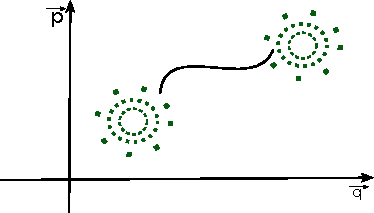
\includegraphics[width = 0.7\textwidth]{Figures/Cap 5/States_Layer 1.pdf}
            \caption{Representation of the evolution of states of a $N$ particles in the phase space.}
            \label{fig:StatesPhase}
        \end{figure}

        In the figure \ref{fig:StatesPhase} we see the evolution of the system but not always look like that, this is only a representation, currently it is more complex the evolution. We can define a distribution function of probability $f$ which tell us the probability to finde the system of $N$ particles in a given state, thus:

        \begin{equation}
            f = f(\Vec{q_1},\Vec{q_2},...,\Vec{q_N},\Vec{p_1},..,\Vec{p_n},t) = f(\Vec{q_i},\Vec{p_i},t)\;,
        \end{equation}

        If the particles are of the same species the function $f$ is normalizade, otherwise it is equal to $N$.
        
        \begin{equation}
            \int f(\Vec{q_i},\Vec{p_i},t)dv = 1\;\;dv = \prod_{i=1}d^3q_id^3p_i
        \end{equation}

        \begin{myteo}
            \textbf{Liouville's theorem:} The volumen of states in the phase space which evolves hamiltonianly from an initial time to a final time is constant, then the states volume is incompressible.
        \end{myteo}

        Lets consider this infinitesimal transformations:

        \begin{equation*}
            q_i \rightarrow q_i + dq_i \;\;\; p_i \rightarrow p_i + dp_i
        \end{equation*}

        Considering the time variations, we've got:

        \begin{equation}\label{eq:qibar}
            q_i \rightarrow q_i + \Dot{q_i}dt = q_i + \frac{\partial H}{\partial p_i}dt = \Bar{q}_i
        \end{equation}

        \begin{equation}\label{eq:pibar}
            p_i \rightarrow p_i + \Dot{p_i}dt = p_i - \frac{\partial H}{\partial q_i}dt = \Bar{p}_i
        \end{equation}

        Now, we want to analyze the volume of states before and after the transformations, so let $dV$ and $d\Bar{V}$ be the volumes of the states befores and after the transformations respectively, then:

        \begin{equation*}
            dV = \prod_{i=1}d^3q_id^3p_i \;\;\; d\Bar{V} = \prod_{i=1}d^3\Bar{q}_id^3\Bar{p}_i
        \end{equation*}

        But from the equations \ref{eq:qibar} and \ref{eq:pibar} we can see that in the volume after the transformation $d\Bar{V}$ appear a Jacobian $d\Bar{V} = det(J)dV$ related to a Jacobian matrix $J$:

        \begin{equation*}
            J = \begin{bmatrix}
                \frac{\partial \Bar{q}_i}{\partial q_j} & \frac{\partial \Bar{q}_i}{\partial p_j}\\

                \frac{\partial \Bar{p}_i}{\partial q_j} & \frac{\partial \Bar{p}_i}{\partial p_j}
            \end{bmatrix}
        \end{equation*}

        \begin{equation}
            det(J) =
            det 
            \begin{pmatrix}
                \delta_{ij} + \frac{\partial^2H}{\partial p_i \partial q_j}dt & \frac{\partial^2 H}{\partial p_j \partial p_i}dt \\

                - \frac{\partial^2 H}{\partial q_j \partial q_i} & \delta_{ij} - \frac{\partial^2 H}{\partial p_j \partial q_i}
            \end{pmatrix}\;,
        \end{equation}

        \begin{equation}
            det(J) = 1 + \sum_{ij}\left(\frac{\partial^2 H}{\partial q_j \partial p_i} - \frac{\partial^2 H}{\partial q_i \partial p_j} \right)dt + \mathcal{O}(dt^2) = 1 + \mathcal{O}(dt^2) \;,
        \end{equation}

        Wee can see that the Jacobian is constant, and because it is constant the \textbf{volume keeps constant.}Because the number of particles must be conserved there must be a continuity equation, and we can define the number of particles $N$ in terms of the distribution function $f$ and the volume, because $f$ is kind of a density, so:

        \begin{equation}
            N = f(\Vec{q}_i,\Vec{p}_pi,t)V
        \end{equation}

        \begin{equation}\label{eq:BoltzmannContinuity}
            \frac{\partial f}{\partial t} + \frac{\partial}{\partial \Vec{q}_i}\cdot (f\Dot{\Vec{q}}_i) + \frac{\partial}{\partial \Vec{p}_i}\cdot(f\Dot{\Vec{p}}_i) = 0
        \end{equation}

        The equation \ref{eq:BoltzmannContinuity} is in fact, the Boltzmann's equation. Now, using the Hamilton's equations the Boltzmann equation  \ref{eq:BoltzmannContinuity} becomes:

        \begin{equation*}
            \frac{\partial f}{\partial t} + \frac{\partial}{\partial \Vec{q}_i}\cdot (f\frac{\partial H}{\partial \Vec{p}_i}) - \frac{\partial}{\partial \Vec{p}_i}\cdot(f\frac{\partial H}{\partial \Vec{q}_i}) = 0
        \end{equation*}

        \begin{equation}
            \frac{\partial f}{\partial t} + \frac{\partial f}{\partial q_i}\frac{\partial H}{\partial p_i} - \frac{\partial f}{\partial p_i}\frac{\partial H}{\partial q_i} =
        \end{equation}

        \begin{equation}\label{eq:LiouvilleEq}
            \frac{\partial f}{\partial t} = \{H,f\}
        \end{equation}

        The equation \ref{eq:LiouvilleEq} is not only a particular case of the Boltzmann equations, it is the Liouville's equation which is strictly related to the Poisson's bracket, is like defining a general partition function. For a distribution functions in equilibrium we've got:

        \begin{equation}
            \{H,f\} = 0
        \end{equation}

        An obvious solution would be a functional of $H$, like the Boltzmann's distribution function $f \alpha e^{-\beta H}$

        \begin{equation}
            \{H,f\} = \frac{\partial H}{\partial \Vec{q}_i}\cdot \frac{\partial H}{\partial \Vec{p}_i}\frac{df}{dH} - \frac{\partial H}{\partial \Vec{p}_i}\cdot \frac{\partial H}{\partial \Vec{q}_i}\frac{df}{dH} = 0
        \end{equation}

        The BBGKY hierarchy doesn't solve the problem but allows us to visualize the problem in a more easy or correct way. How would be the distribution function for a particle, or two, or s particles?The function $f$ and their individual or joint probabilities are related by:

        \begin{equation}
            f_1(\Vec{q},\Vec{p},t) = <\sum_{i=1}^N \delta^3(\Vec{q}-\Vec{q}_i)\delta^3(\Vec{p}-\Vec{p}_i)>\;,
        \end{equation}

        \begin{equation}
            f_1(\Vec{q},\Vec{p},t) = N \int f(\Vec{q},\Vec{q}_2,...,\Vec{q}_N,\Vec{p},\Vec{p}_2,...,\Vec{p}_N,t)\prod_{i=2}^Nd^3q_id^3p_i
        \end{equation}

        \begin{equation}
            f_2(\Vec{q}_1 , \Vec{q}_2,\Vec{p}_1, \Vec{p}_2 ,t) = N(N-1) \int f(\Vec{q}_1,\Vec{q}_2,...,\Vec{q}_N,\Vec{p}_1,\Vec{p}_2,...,\Vec{p}_N,t)\prod_{i=3}^Nd^3q_id^3p_i
        \end{equation}

        \begin{equation}
            f_s(\Vec{q}_1 ,..., \Vec{q}_s,\Vec{p}_1, ..., \Vec{p}_s ,t) = \frac{N!}{(N-s)!} \int f(\Vec{q}_1,\Vec{q}_2,...,\Vec{q}_N,\Vec{p}_1,\Vec{p}_2,...,\Vec{p}_N,t)\prod_{i=s+1}^Nd^3q_id^3p_i
        \end{equation}

        This is the well-known BBGKY hierarchy, the first distribution function $f_1$ corresponds to the Boltzmann's formulation, the second one to the Bogoliubov and so on. It is obvious that $f_s$ contains the information of all the other distribution functions of lower order, and also must interact with the system just to its side, in terms of a Hamiltonian, there is a Hamiltonian of interaction between the s-level and the 
        (s+1)-level, as follows:

        \begin{equation}
            H = H_s + H_{N-s} + H'
        \end{equation}

        $H'$ corresponds to the interaction between the s-particles and the $N-s$ particles:

        \begin{equation}
            H = \sum_{n=1}^s \left[\frac{p^2}{2m} + V(\Vec{q}_n) \right] + \frac{1}{2}\sum_{n,m = 1}^s U(\Vec{q}_n - \Vec{q}_m)\;,
        \end{equation}

        \begin{equation}
            H = \sum_{i = s+1}^N \left[\frac{p^2}{2m} + V(\Vec{q}_n) \right] + \frac{1}{2}\sum_{i,j = s+1}^N U(\Vec{q}_i - \Vec{q}_j)\;,
        \end{equation}

        \begin{equation}
            H' = \sum_{n=1}^s\sum_{i = s+1}^N U(\Vec{q}_n - \Vec{q}_i)\;.
        \end{equation}

    From now on, we're going to analyze the time evolution of the $s-th$ probability function to give rise an important conclusion \textbf{the particles at the s-level only interacts with the particles of the s+1-level}. Thus:

    \begin{equation}
        \frac{\partial f_s}{\partial t} = \frac{N!}{(N-s)!}\int\frac{\partial f}{\partial t}\prod_{i = s+1}^Nd^3q_id^3p_i\;,
    \end{equation}

    \begin{equation*}
        \frac{\partial f_s}{\partial t} = \frac{N!}{(N-s)!}\int\{H,f\}\prod_{i = s+1}^N d^3q_id^3p_i = - \frac{N!}{(N-s)!}\int \{f,H_s + H_{N-s} + H'\}\prod_{i = s+1}^Nd^3q_id^3p_i\;,
    \end{equation*}

    \begin{align}
        \frac{\partial f_s}{\partial t} = -\frac{N!}{(N-s)!}\int\{f,H_s\}\prod_{i=s+1}^Nd^3q_id^3p_i - \frac{N!}{(N-s)!}\int\{f,H_{N-s}\}\prod_{i=s+1}^Nd^3q_id^3p_i \\
        - \frac{N!}{(N-s)!}\int\{f,H'\}\prod_{i=s+1}^Nd^3q_id^3p_i\;.
    \end{align}

    This is more accurate way to visualize the hierarchy, to determine this three integrals, we're going to calle them $T_1$ , $T_2$ and $T_3$ respectively.

    \begin{equation*}
        T_1 = -\frac{N!}{(N-s)!}\int\{f,H_s\}\prod_{i=s+1}^Nd^3q_id^3p_i = -\left\{\frac{N!}{(N-s)!}\int f\prod_{i=s+1}^Nd^3q_id^3p_i  , H_s\right\}
    \end{equation*}

    \begin{equation}\label{eq:T1}
        T_1 = \{H_s,f_s\}
    \end{equation}

    This was integrated in that way because $H_s$ is constant in that interval, because we're integrating from $s+1$ to $N$.

    \begin{equation*}
        T_2 = - \frac{N!}{(N-s)!}\int\{f,H_{N-s}\}\prod_{i=s+1}^Nd^3q_id^3p_i = \frac{N!}{(N-s)!}\int\left[\frac{\partial H_{N-s}}{\partial q_j}\frac{\partial f}{\partial p_j} - \frac{\partial H_{N-s}}{\partial p_j}\frac{\partial f}{\partial q_j} \right]\prod_{i=s+1}^Nd^3q_id^3p_i\;,
    \end{equation*}

    \begin{equation*}
        T_2 = \frac{N!}{(N-s)!}\int\left[\frac{\partial f}{\partial p_j} \cdot \left(\frac{\partial V}{\partial q_j} + \frac{1}{2}\sum_{k=s+1}^N\frac{\partial U(\Vec{q}_j - \Vec{q}_k)}{\partial q_j} \right) - \frac{\partial f}{\partial q_j}\cdot \frac{\Vec{P}_j}{m}\right]\prod_{i=s+1}^Nd^3q_id^3p_i
    \end{equation*}

    And integrating by parts the second integral $T_2$ becomes zero, therefore we must focus on the third integral $T_3$:

    \begin{equation*}
        T_3 = - \frac{N!}{(N-s)!}\int\{f,H'\}\prod_{i=s+1}^Nd^3q_id^3p_i = \frac{N!}{(N-s)!}\int\left[\frac{\partial H'}{\partial q_j}\cdot\frac{\partial f}{\partial p_j} - \frac{\partial H'}{\partial p_j}\cdot\frac{\partial f}{\partial q_j}\right]\prod_{i=s+1}^Nd^3q_id^3p_i\;,
    \end{equation*}

    But $H'$ doesn't depend explicitly on $\Vec{P}_i$ son the second term of the Poisson's brackets vanishes, then:

    \begin{equation*}
        T_3 = \frac{N!}{(N-s)!}\int\left[\sum_{n=1}^s \frac{\partial f}{\partial P_n}\cdot \sum_{j = s+1}^N \frac{\partial U(\Vec{q_n} - \Vec{q_j})}{\partial q_n} + \sum_{j=s+1}^N\frac{\partial f}{\partial P_j}\cdot \sum_{n=1}^s\frac{\partial U(\Vec{q_n}-\Vec{q_j})}{\partial q_j} \right]\prod_{i=s+1}^Nd^3q_id^3p_i
    \end{equation*}

    Using integration by parts on the second term of the Poisson's bracket we will obtain that term vanishes, then:

    \begin{equation}
        T_3 = \frac{N!}{(N-s)!}\int \sum_{n=1}^s \frac{\partial f}{\partial \Vec{P}_n}\cdot \sum_{j=s+1}^N\frac{\partial U(\Vec{q_n} - \Vec{q_j}}{\partial \Vec{q}_n}\prod_{i=s+1}^Nd^3q_id^3p_i\;,
    \end{equation}

    In general, the \textbf{BBGKY hierarchy equation is:}

    \begin{equation}
        \frac{\partial f_s}{\partial t} - \{H_s,f_s\} = T_3
    \end{equation}

    To give a better form of this equation lets analyze the Liouville's distribution function, to do this lets analyze the "momentum gradient" of the $s-th$ and $s+1-th$ levels:

    \begin{equation}
        \frac{\partial f_s}{\partial \Vec{P}} = \frac{N!}{(N-s)!}\int \frac{\partial f}{\partial \Vec{p}_n}\prod_{i=s+1}^Nd^3q_id^3p_i\;,
    \end{equation}

    \begin{equation}
        \frac{\partial f_{s+1}}{\partial \Vec{p}_n} = \frac{N!}{(N-s)!}\int \frac{\partial f}{\partial \Vec{p}_n}\prod_{i=s+1}^Nd^3q_id^3p_i\;.
    \end{equation}

    But we can give it another integral form taking advantage  that the particles are indistinguishable:

    \begin{equation*}
        T_3 = \frac{N!}{(N-s)!}(N-s)\int \sum_{n=1}^s \frac{\partial f}{\partial \Vec{p}_n}\cdot \frac{\partial U(\Vec{q}_n - \Vec{q}_{s+1})}{\partial \Vec{q}_n}\prod_{i=s+1}^Nd^3q_id^3p_i\;,
    \end{equation*}

    \begin{equation*}
        T_3 = \frac{N!}{(N-s)!}\sum_{n=1}^s\int d^3q_{s+1}d^3p_{s+1} \frac{\partial U(\Vec{q}_n - \Vec{q}_{s+1})}{\partial \Vec{q}_n}\cdot \left(\prod_{i=s+2}^Nd\frac{\partial f}{\partial \Vec{p}_n}d^3q_id^3p_i \right)\;,
    \end{equation*}

    \begin{equation}
        T_3 = \sum_{n=1}^s\int\frac{\partial U(\Vec{q}_n - \Vec{q}_{s+1})}{\partial \Vec{q}_n}\cdot \frac{\partial f_{s+1}}{\partial \Vec{p}_n}d^3q_{s+1}d^3p_{s+1}\;.
    \end{equation}

    \textit{The $s$ particles interact with the $s+1$ particles and not with the $s+2$ or $s+3$ or $s+k$.} In total, we have the following equations for a \textbf{hamiltonian system with $N$ indistinguishable particles:}

    \begin{enumerate}
        \item 
        \begin{equation}
            \frac{\partial f_s}{\partial t} - \{H_s,f_s\} = \left(\frac{\partial f_s}{\partial t} \right)_{coll}\;,
        \end{equation}

        \item 

        \begin{equation}
            \left(\frac{\partial f_s}{\partial t} \right)_{coll} = \sum_{n=1}^s\int\frac{\partial U(\Vec{q}_n - \Vec{q}_{s+1})}{\partial \Vec{q}_n}\cdot \frac{\partial f_{s+1}}{\partial \Vec{p}_n}d^3q_{s+1}d^3p_{s+1}\;,
        \end{equation}

        \item 
        \begin{equation}
            f_s(\Vec{q}_1,...,\Vec{q}_s,\Vec{p}_1,...,\Vec{p}_s,t)= \frac{N!}{(N-s)!}\int f(\Vec{q}_i,\Vec{p}_i,t)\prod_{i=s+1}d^3q_id^3p_i\;.
        \end{equation}
    \end{enumerate}


    \subsection{Boltzmann equation: The theory of one particle}

    
    Using all the development previously done we can arrive to the Boltzmann equation an the theory of one particle. 

    \begin{equation}\label{eq:f1}
        f(\Vec{q},\Vec{p},t) = N\int f(\Vec{q}_i,\Vec{p}_i,t)\prod_{i=2}^Nd^3q_id^3p_i\;,
    \end{equation}

    \begin{equation}
        \frac{\partial f_1}{\partial t} - \{H_1,f_1\} = \left(\frac{\partial f_1}{\partial t}\right)_{coll} = \int \frac{\partial U(\Vec{q} - \Vec{q}_2)}{\partial \Vec{p}} \cdot \frac{\partial f_2}{\partial \Vec{p}}d^3p_2d^3q_2\;.
    \end{equation}


    From the equation \ref{eq:f1} we can already rise some physical interpretations, if we integrate \ref{eq:f1} we won't get $1$ we'll get $N$ this means, that in fact this is not a theory of one particle this is the theory of one of many particles, in fact there are still $N$ particles evolving, we're only focusing one but still there is a whole dynamics. To calculate the term of collisions we must find $f_2$, thus:

    \begin{equation}
        f_2(\Vec{q_1},\Vec{q}_2,\Vec{p}_1,\Vec{p}_2,t) = N(N-1)\int f(\Vec{q}_i,\Vec{p}_i,t)\prod_{i=3}^Nd^3q_id^3p_i\;.
    \end{equation}


    From \ref{eq:f1} we can obtain so many properties of the system, such as:

    \begin{itemize}
        \item The number density $n$:
        \begin{equation}
            n(\Vec{q},t) = \int f_1(\Vec{q},\Vec{p},t)d^3p\;.
        \end{equation}

        \item The speed $\Vec{V}$:

        \begin{equation}
            \Vec{V}(\Vec{q},\Vec{p},t) = \int \frac{\Vec{P}}{m}f_1(\Vec{q},\Vec{p},t)d^3p\;.
        \end{equation}

        \item  The energy flux $\xi$:
        \begin{equation}
            \xi (\Vec{q},t) = \int \frac{\Vec{P}}{m}E(\Vec{p})f_1(\Vec{q},\Vec{p},t)d^3p\;.
        \end{equation}
    \end{itemize}


    
    \appendix
    
    \section{Sommerfeld quantization}\label{APX:Sommerfeld}

        The Bohr model was successful in predicting the outcomes of experiments, but the fundamental postulates it was based on remained mysterious. One major mystery was how Bohr's quantization of an electron's orbital angular momentum in a circular orbit related to Planck's quantization of the total energy of an entity, like an electron, in simple harmonic motion. In 1916, Wilson and Sommerfeld shed some light on this by outlining a set of rules for quantizing any physical system with periodic time functions as coordinates. These rules included both Planck and Bohr's quantizations as special cases. Essentially, for any physical system with periodic time functions as coordinates, there is a quantum condition for each coordinate, that is the following:

        \begin{equation}\label{eq:QSomm}
            \oint pdq = n_qh
        \end{equation}

        Where ${q,p}$ are conjugated pairs and $n_q$ is a quantum number which takes on integral values, and means that the integration is taken over one period of the coordinate q. With this we can get the Planck's quantization of the mechanical oscillators, let $E$ the energy of a harmonic oscillator:

        \begin{equation*}
            E = T + V = \frac{1}{2}mv^2 + \frac{1}{2}kx^2 = \frac{p^2}{2m} + \frac{1}{2}kx^2
        \end{equation*}

        \begin{equation}
            \frac{p^2}{2mE} + \frac{x^2}{2E/k} = 1
        \end{equation}

        That is the equation of an ellipse, with this representation in a phase space $p vs x$ we can calculate easily the integral \ref{eq:QSomm}:

        \begin{equation*}
            \oint pdq = n_qh = 2\pi E \sqrt{\frac{m}{k}} = \frac{2\pi E}{2\pi \nu}
        \end{equation*}

        \begin{equation}
            E = nh\nu \;[J]
        \end{equation}

        Note that the allowed energy states of oscillation are represented by a series of ellipses in phase space, the area enclosed between successive ellipses always being $h$. We find that the classical situation corresponds to $h \rightarrow 0$, all values of E and hence all ellipses being allowed if that were true.\\

        We can also deduce the Bohr's quantization of angular momentum so let an electron moving in a circular orbit of radius $r$ has an angular momentum, $mvr = L$, which is constant. The angular coordinate is $\theta$, which is a periodic function of the time. That is $\theta vs t$ is a function increasing linearly from zero to $2\pi$ in one period and repeating this pattern in each succeeding period. The quantization rule is:

        \begin{equation}
            \oint L d\theta = L \int_0^{2\pi}d\theta = nh 
        \end{equation}

        \begin{equation}
            L = n\hbar
        \end{equation}

        A more physical interpretation of the Bohr quantization rule was given in $1924$ by DeBroglie. The Bohr quantization of angular momentum can be written as: 

        \begin{equation*}
            L = mvr = pr = n\hbar  \;\; p = \frac{k}{\hbar}=\frac{h}{\lambda}
        \end{equation*}

        \begin{equation*}
            L = \frac{hr}{\lambda} = n\hbar \rightarrow 2\pi r = n\lambda
        \end{equation*}

        Where $p$ is the linear momentum of an electron in an allowed orbit of radius $r$. Therefore, only certain orbits are allowed for the electron, where the circumference of the orbit must be an exact multiple of the de Broglie wavelength. This means that as the electron moves at a constant speed in its orbit around the nucleus, it also has an associated wave with a wavelength specified by the de Broglie postulates. When the electron completes a cycle around the nucleus, the wave associated with the electron will restore itself. If the orbit circumference is equal to an integer of the wavelength, then the resulting overlapping waves from the completed several courses around the nucleus will be in the same phase. However, if the orbit circumference is not equal to an integer of the wavelength, the overlapping waves will cancel each other out, and the accompanying wave in this case will be zero. 


    \section{Laplacian in spherical coordinates}

    The Laplacian is an important mathematical operator used in many areas of physics, including electromagnetism and fluid dynamics. It is often written in terms of partial derivatives, and its form can depend on the coordinate system being used. Here is the general expression for the Laplacian in arbitrary coordinates:
    \begin{equation*}
        \nabla^2 f = \frac{1}{\sqrt{g}} \sum_{i,j=1}^n \frac{\partial}{\partial x^i} \left( \sqrt{g} g^{ij} \frac{\partial f}{\partial x^j} \right)
    \end{equation*}

    \begin{equation*}
        \nabla^2 f = \frac{1}{r^2} \frac{\partial}{\partial r} \left( r^2 \frac{\partial f}{\partial r} \right) + \frac{1}{r^2 \sin \theta} \frac{\partial}{\partial \theta} \left( \sin \theta \frac{\partial f}{\partial \theta} \right) + \frac{1}{r^2 \sin^2 \theta} \frac{\partial^2 f}{\partial \phi^2}
    \end{equation*}
    
{\bibliographystyle{apalike}}
\bibliography{bibliografia.bib}

\end{document}